\documentclass[twocolumn,5p]{elsarticle}
\pdfoutput=1
\usepackage{tikz}
\usepackage{comment}
\usepackage{framed,graphicx}
\usepackage{multirow}
\usepackage{rotating}
\usepackage{amsmath}
\usepackage{bigstrut}
\usepackage{color}
\usepackage{graphics}
\usepackage{eqparbox}
\usepackage{graphics}
\usepackage{colortbl}
\usepackage{paralist}

\usepackage{caption}
%\usepackage{times}
\usepackage{mathptmx} 
\usepackage{courier}
\usepackage{balance}
\usepackage{picture}
\usepackage{algorithm}
\usepackage{algorithmicx}
\usepackage{algpseudocode}
\usepackage[export]{adjustbox}
\definecolor{lightgray}{gray}{0.8}
\definecolor{darkgray}{gray}{0.6}
\definecolor{lavenderpink}{rgb}{0.98, 0.68, 0.82}
\definecolor{celadon}{rgb}{0.67, 0.88, 0.69}
\renewcommand{\algorithmicrequire}{\textbf{Input:}}
\renewcommand{\algorithmicensure}{\textbf{Output:}}
%%% graph
\newcommand{\crule}[3][darkgray]{\textcolor{#1}{\rule{#2}{#3}}}

\newcommand{\quart}[4]{\begin{picture}(80,4)%1
	{\color{black}\put(#3,2){\circle*{4}}\put(#1,2){\line(1,0){#2}}}\end{picture}}

\definecolor{Gray}{gray}{0.95}
\definecolor{LightGray}{gray}{0.975}


%% timm tricks
\newcommand{\bi}{\begin{itemize}[leftmargin=0.4cm]}
	\newcommand{\ei}{\end{itemize}}
\newcommand{\be}{\begin{enumerate}}
	\newcommand{\ee}{\end{enumerate}}

\usepackage[shortlabels]{enumitem}
\usepackage{url}

\definecolor{steel}{rgb}{.11, .11, .7}
\definecolor{Gray}{rgb}{0.88,1,1}
\definecolor{Gray}{gray}{0.85}
\usepackage[framed]{ntheorem}
\usetikzlibrary{shadows}
\theoremclass{Lesson}
\theoremstyle{break}

% inner sep=10pt,
\tikzstyle{thmbox} = [rectangle, rounded corners, draw=black,
fill=Gray!40,  drop shadow={fill=black, opacity=1}]
\newcommand\thmbox[1]{%
	\noindent\begin{tikzpicture}%
	\node [thmbox] (box){%
		\begin{minipage}{.94\textwidth}%
		\vspace{-2mm}#1\vspace{-3mm}%
		\end{minipage}%
	};%
	\end{tikzpicture}}

\let\theoremframecommand\thmbox
\newshadedtheorem{lesson}{Result}



\begin{document}
\begin{frontmatter}

\title{What is  Wrong with
Topic Modeling?\\ (and How to Fix it Using Search-based SE)}



\author[label1]{Amritanshu Agrawal\corref{cor1}}
\address[label1]{Department of Computer Science, North Carolina State University, Raleigh, NC, USA}

\cortext[cor1]{Corresponding author: Tel: +1-919-637-0412 (Amritanshu)}

\ead{aagrawa8@ncsu.edu}
\ead[url]{http://ai4se.net/}

\author[label1]{Wei Fu\corref{cor1}}
\ead{wfu@ncsu.edu}

\author[label1]{Tim Menzies\corref{cor1}}
\ead{tim.menzies@gmail.com}

\begin{abstract}

\noindent
\textbf{Context:} Topic Modeling finds
  human-readable structures in large sets of unstructured data. A widely used topic modeler is Latent Dirichlet Allocation. When run on different datasets, LDA suffers from ``order effects'' i.e. 
 different distributions are generated if the training data was shuffled into a different order. Such order effects introduce a systematic error for any study. This error can relate to all kinds of machine learning problem where LDA is being used.
 
 \noindent
\textbf{Objective:} To provide a method in which distributions generated by LDA are more stable and can be used for further analysis.

 \noindent
\textbf{Method:} We introduce LDADE, a Search-Based Software Engineering tool that tunes LDA's parameters using DE 
(Differential Evolution).

\noindent
\textbf{Evaluation:} 
LDADE is evaluated on data from a programmer
information exchange site (StackOverflow), title and abstract text of thousands
of Software Engineering (SE) papers, and software defect reports from NASA. Results were collected
across different implementations of LDA (Python+Scikit-Learn, Scala+Spark); across
different platforms (Linux, Macintosh) and for different kinds of LDAs (the
traditional VEM method, or using Gibbs sampling). 

\noindent
\textbf{Results:}
LDA suffers from order effects and our LDADE was able to stabilize the distribution. It gave improved performances for supervised as well as unsupervised learning.

\noindent
\textbf{Conclusion}
In all tests, the pattern was
the same: LDADE's tunings dramatically reduces cluster instability. And in turn reduces the error in Supervised and Unsupervised machine learning problem. The implications of this study for other software analytics tasks is now an open and pressing issue. In how many domains can search-based SE dramatically improve software analytics? 
\end{abstract}

\begin{keyword}
Topic modeling, Stability, LDA, tuning, differential evolution.
\end{keyword}

\end{frontmatter}



\section{Introduction}
\label{sect: intro}
The current great challenge in software analytics is understanding unstructured data. As shown in Figure~\ref{fig: data}, most of the planet's 1600 Exabytes of data does not appear in structured sources (databases, etc)~\cite{nadkarni2014structured}. Rather it is {\em unstructured} data, often in free text, and found in word processing files, slide presentations, comments, etc etc. 

Such unstructured data does not have a pre-defined data model and is typically text-heavy. Finding insights among unstructured text is  difficult unless we can search, characterize, and classify the textual data in a meaningful way. One of the common techniques for finding related topics within unstructured text (an area called topic modeling) is Latent Dirichlet Allocation (LDA)~\cite{blei2003latent}.
Topic modeling is widely used in Software Engineering and many papers in recent years have reported  topic modeling results at numerous SE venues (see  Table~\ref{tab:venues} and ~\ref{tbl:survey2}). These two tables show how important LDA has been in various SE tasks and most of them are recently published.

\begin{figure}[!t]
  \captionsetup{justification=centering}
  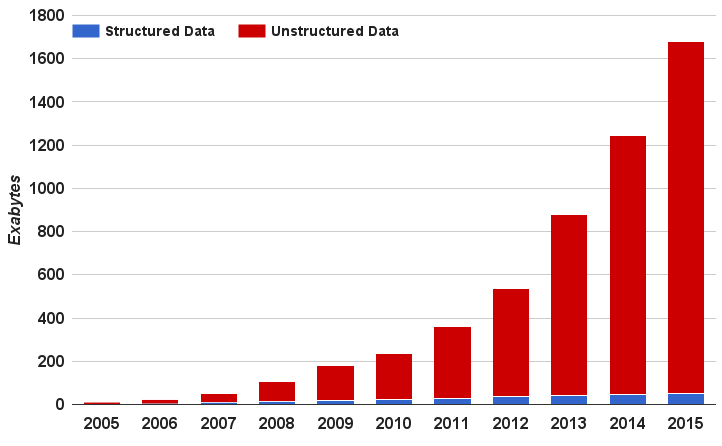
\includegraphics[width=\linewidth]{./fig/data.png}
  \caption{Data Growth 2005-2015. From~\cite{nadkarni2014structured}.}
  \label{fig: data}
\end{figure}

Topic models built by LDA are non-deterministic in behaviour. Due to non-determinism, topics generated by LDA are not stable~\cite{oliveto2010equivalence, barua2014developers}. It learns the various distributions which is a problem of Bayesian inference~\cite{blei2003latent}. We are talking about model instability itself which further affects the results. Many industries, working on a product development in text analytics have been widely using it. They want better results in their product. Menzies et al~\cite{menzieslocal} showed how model instability can give rise to large effort estimations across various projects. And we do need to avoid these large effort estimations.

LDA takes certain set of parameters which try to take us closer to good cluster distributions. But it is an art to find the right parameters setting that control the choices within a data miner. But it is very impractical to get the right parameters settings due to larger search space of configurations. Nevertheless, we rarely tuned LDA since we reasoned that a LDA’s default tunings have been well-explored by the developers of those algorithms (in which case tuning would not lead to stable topic models). Due to larger search space of configurations, it is not even feasible to find such tunings. And that is why, LDA is usually used with off-the-shell default parameters. Many researchers have agreed to the idea of using different configurations in LDA. But, we have seen rare work done when it comes to tune the important parameters of LDA.

\begin{table}[!t]
\renewcommand\arraystretch{0.8}
\begin{center}
\scriptsize
\begin{tabular}{|c|l|c|}
\hline
\begin{tabular}[c]{@{}c@{}}\textbf{Venue}\end{tabular} & \begin{tabular}[c]{@{}c@{}}\textbf{Full Name}\end{tabular}     & \multicolumn{1}{l|}{\textbf{Count}} \\ \hline
ICSE & International Conference on Software Engineering  & 4  \\ \hline
\begin{tabular}[c]{@{}c@{}}CSMR-\\WCRE\\ / SANER \end{tabular}   & \begin{tabular}[c]{@{}l@{}}International Conference on Software Maintenance,\\ Reengineering, and Reverse Engineering / International \\Conference on Software Analysis,Evolution, and \\Reengineering\end{tabular} & 3  \\ \hline
\begin{tabular}[c]{@{}c@{}}ICSM\\ / ICSME\end{tabular}   & \begin{tabular}[c]{@{}l@{}}International Conference on Software Maintenance / \\International Conference on Software Maintenance and \\Evolution \end{tabular}  & 3\\ \hline
ICPC & International Conference on Program Comprehension  & 4  \\ \hline
ASE      & \begin{tabular}[c]{@{}l@{}}International Conference on Automated Software\\ Engineering  \end{tabular} & 3  \\ \hline
ISSRE      & \begin{tabular}[c]{@{}l@{}}International Symposium on Software Reliability\\ Engineering \end{tabular} & 2  \\ \hline
MSR      & \begin{tabular}[c]{@{}l@{}}International Working Conference on Mining \\Software Repositories \end{tabular} & 8  \\ \hline
OOPSLA  & \begin{tabular}[c]{@{}l@{}}International Conference on Object-Oriented \\Programming, Systems, Languages, and Applications \end{tabular}  & 1 \\ \hline
FSE/ESEC  &  \begin{tabular}[c]{@{}l@{}}International Symposium on the Foundations of Software \\Engineering / European Software Engineering Conference \end{tabular}  & 1                                    \\ \hline
TSE                                 & IEEE Transaction on Software Engineering   & 1                                     \\ \hline
IST                                 & Information and Software Technology                                 & 3                                       \\ \hline
SCP                                 & Science of Computer Programming                               & 2                                       \\ \hline
ESE                                 & Empirical Software Engineering                         & 4                                       \\ \hline
\end{tabular}
\end{center}
\caption{SE Venues that publish  on Topic Modeling.}
\label{tab:venues}
\end{table}

Researchers use topic models mostly in either of two ways.
Firstly,
topics may be used as {\em feature selector} that finds useful inputs
which are then used by, say, a classifier to characterize different kinds of software (e.g. buggy or not~\cite{chen2016topic}).
In this mode, no human ever need to read the generated topics but the cluster distribution still suffers from instabilities and they pose problem in classification tasks. 

Secondly, researchers may present and reflect on the generated topics in order to
  offer some insight into the structure of the data.  In this second mode,
  researchers present and discuss the specifics of the generated topics in order
  to defend particular conclusions. A case study related to this problem is performed which was similar to Barua et al \cite{barua2014developers}. 

\renewcommand\arraystretch{1.2}
\begin{table*}[!t]
\tiny
  \centering
    \begin{tabular}{|c@{~}|c@{~}|c@{~}|c@{~}|c@{~}|c@{~}|c@{~}|p{7.5cm}@{~}|p{2.5cm}|}
        \hline 
        \begin{tabular}[c]{@{}c@{}}\textbf{Reference} \\\textbf{ID}\end{tabular} & \textbf{Year} & \textbf{Citations} & \textbf{Venues} & \begin{tabular}[c]{@{}c@{}}\textbf{Mentions} \\\textbf{instability} \\\textbf{in LDA?} \end{tabular} &\begin{tabular}[c]{@{}c@{}} \textbf{Talks about} \\\textbf{using-off-the} \\\textbf{shell parameters?}\end{tabular}&\begin{tabular}[c]{@{}c@{}} \textbf{Does} \\\textbf{tuning?}\end{tabular} & \multicolumn{1}{c|}{Conclusion}  & \multicolumn{1}{c|}{Tasks / Use cases}\\ \hline
        ~\cite{rao2011retrieval} & 2011 & 112 & WCRE & Y & Y & N & \begin{tabular}[c]{@{}l@{}}Explored Configurations without any explanation. \end{tabular} & \begin{tabular}[c]{@{}l@{}}Bug Localisation\end{tabular}\\ [0.5ex]\hline
        ~\cite{oliveto2010equivalence} & 2010 & 108 &MSR& Y & Y & N & \begin{tabular}[c]{@{}l@{}}Explored Configurations without any explanation. Reported their results using multiple experiments.\end{tabular}& \begin{tabular}[c]{@{}l@{}}Traceability Link recovery\end{tabular}\\ [0.5ex]\hline
        ~\cite{barua2014developers} &2014& 96 & ESE & Y & Y & N  & \begin{tabular}[c]{@{}l@{}}Explored Configurations without any explanation. Choosing right set of parameters is a difficult task.\end{tabular}& \begin{tabular}[c]{@{}l@{}}StackOverflow Q\&A data analysis\end{tabular}\\ [0.5ex]
        \hline
        ~\cite{panichella2013effectively} & 2013&75&ICSE & Y & Y & Y  & \begin{tabular}[c]{@{}l@{}}Uses GA to tune parameters. They determine the near-optimal configuration for LDA in the context \\of only some important SE tasks.\end{tabular}& \begin{tabular}[c]{@{}l@{}}Finding near-optimal configurations\end{tabular}\\ [0.5ex]
        \hline
        ~\cite{galvis2013analysis} &2013& 61 &ICSE& Y & Y & N  & \begin{tabular}[c]{@{}l@{}}Explored Configurations without any explanation.\end{tabular}& \begin{tabular}[c]{@{}l@{}}Software Requirements Analysis\end{tabular}\\ [0.5ex]
        \hline
        ~\cite{hindle2011automated} &2011& 45 & MSR & Y & Y & N  & \begin{tabular}[c]{@{}l@{}}They validated the topic labelling techniques using multiple experiments.\end{tabular}& \begin{tabular}[c]{@{}l@{}}Software Artifacts Analysis\end{tabular}\\ [0.5ex]
        \hline
        ~\cite{guzman2014users} & 2014 & 44 &RE& Y & Y & N  & \begin{tabular}[c]{@{}l@{}}Explored Configurations without any explanation.\end{tabular}& \begin{tabular}[c]{@{}l@{}}Requirements Engineering\end{tabular}\\ [0.5ex]
        \hline
        ~\cite{thomas2011mining} &2011& 44 &ICSE & Y & Y & N  & \begin{tabular}[c]{@{}l@{}}Open issue to choose optimal parameters.\end{tabular}& \begin{tabular}[c]{@{}l@{}}A review on LDA\end{tabular}\\ [0.5ex]
        \hline
        ~\cite{thomas2014studying} & 2014 & 35 &SCP& Y & Y & N  & \begin{tabular}[c]{@{}l@{}}Explored Configurations without any explanation.\end{tabular}& \begin{tabular}[c]{@{}l@{}}Software Artifacts Analysis\end{tabular}\\ [0.5ex]
        \hline
        ~\cite{chen2012explaining} &2012& 35 &MSR & Y & Y & N  & \begin{tabular}[c]{@{}l@{}}Choosing the optimal number of topics is difficult.\end{tabular}& \begin{tabular}[c]{@{}l@{}}Software Defects Prediction\end{tabular}\\ [0.5ex]
        \hline
        ~\cite{thomas2014static} &2014& 31 &ESE& Y & Y & N  & \begin{tabular}[c]{@{}l@{}}Choosing right set of parameters is a difficult task.\end{tabular}& \begin{tabular}[c]{@{}l@{}}Software Testing\end{tabular}\\ [0.5ex]
        \hline
        ~\cite{bajracharya2009mining} &2009 &29 & MSR& Y & Y & N  & \begin{tabular}[c]{@{}l@{}}Explored Configurations without any explanation and accepted to the fact their results were better \\because of the corpus they used.\end{tabular}& \begin{tabular}[c]{@{}l@{}}Software History Comprehension\end{tabular}\\ [0.5ex]
        \hline
        ~\cite{lohar2013improving} &2013& 27 &ESEC/FSE &Y & Y & Y  & \begin{tabular}[c]{@{}l@{}}Explored Configurations using LDA-GA.\end{tabular}& \begin{tabular}[c]{@{}l@{}}Traceability Link recovery\end{tabular}\\ [0.5ex]
        \hline
        ~\cite{binkley2014understanding} &2014& 20 &ICPC& Y & Y & N  & \begin{tabular}[c]{@{}l@{}}Use heuristics to find right set of parameters.\end{tabular}& \begin{tabular}[c]{@{}l@{}}Source Code Comprehension\end{tabular}\\ [0.5ex]
        \hline
        ~\cite{linares2013exploratory} &2013& 20 &MSR& Y & Y & N  & \begin{tabular}[c]{@{}l@{}}In Future, they planned to use LDA-GA.\end{tabular}& \begin{tabular}[c]{@{}l@{}}StackOverflow Q\&A data analysis\end{tabular}\\ [0.5ex]
        \hline
        ~\cite{koltcov2014latent} & 2014 & 15 & WebSci& Y & Y & N  & \begin{tabular}[c]{@{}l@{}}Explored Configurations without any explanation.\end{tabular}& \begin{tabular}[c]{@{}l@{}}Social Software Engineering\end{tabular}\\ [0.5ex]
        \hline
        ~\cite{grant2013using} & 2013 & 13 &SCP& Y & Y & N  & \begin{tabular}[c]{@{}l@{}}Their work focused on optimizing LDA’s topic count parameter.\end{tabular}& \begin{tabular}[c]{@{}l@{}}Source Code Comprehension\end{tabular}\\ [0.5ex]
        \hline
        ~\cite{hindle2012relating} & 2012 & 13 &ICSM& Y & Y & N  & \begin{tabular}[c]{@{}l@{}}Explored Configurations without any explanation (Just with no. of topics).\end{tabular}& \begin{tabular}[c]{@{}l@{}}Software Requirements Analysis\end{tabular}\\ [0.5ex]
        \hline
        ~\cite{fu2015automated} &2015& 6 & IST & Y & Y & N  & \begin{tabular}[c]{@{}l@{}}Explored Configurations without any explanation. Choosing right set of parameters is a difficult task.\end{tabular}& \begin{tabular}[c]{@{}l@{}}Software re-factoring\end{tabular}\\ [0.5ex]
        \hline
        ~\cite{garousi2016citations} &2016& 5 &\begin{tabular}[c]{@{}c@{}}CS Review\end{tabular}& Y & Y & N  & \begin{tabular}[c]{@{}l@{}}Explored Configurations without any explanation.\end{tabular}& \begin{tabular}[c]{@{}l@{}}Bibliometrics and citations analysis\end{tabular}\\ [0.5ex]
        \hline
        ~\cite{le2014predicting} &2014& 5 & ISSRE& N & Y & N  & \begin{tabular}[c]{@{}l@{}}Explored Configurations without any explanation.\end{tabular}& \begin{tabular}[c]{@{}l@{}}Bug Localisation\end{tabular}\\ [0.5ex]
        \hline
        ~\cite{nikolenko2015topic} & 2015 &3 &JIS& Y & Y & N  & \begin{tabular}[c]{@{}l@{}}They improvised LDA into ISLDA which gave stability across different runs.\end{tabular}& \begin{tabular}[c]{@{}l@{}}Social Software Engineering\end{tabular}\\ [0.5ex]
        \hline
        ~\cite{sun2015msr4sm} &2015& 2 &IST& Y & Y & Y  & \begin{tabular}[c]{@{}l@{}}Explored Configurations using LDA-GA.\end{tabular}& \begin{tabular}[c]{@{}l@{}}Software Artifacts Analysis\end{tabular}\\ [0.5ex]
        \hline
        ~\cite{chen2016topic} &2016& 0 &JSS& N & Y & N  & \begin{tabular}[c]{@{}l@{}}Explored Configurations without any explanation. Choosing right set of parameters is a difficult task.\end{tabular}& \begin{tabular}[c]{@{}l@{}}Software Defects Prediction\end{tabular}\\ [0.5ex]
        \hline
\end{tabular}
\caption{A sample of the recent literature on using topic modeling in SE. Note that some of these papers are widely-cited. }
\label{tbl:survey2}
\end{table*}

\renewcommand\arraystretch{1.2}

\begin{table*}[!htbp]
\begin{center}


    \begin{minipage}{.51\textwidth}
        \tiny
  
    \begin{tabular}{|p{6.7cm}@{~}|}
        \hline 
        \multicolumn{1}{|c|}{Top LDA words} \\ \hline
       \begin{tabular}[c]{@{}l@{}}\textbf{Topic Java Programming}: ~string new public int null return privat void java \\ 
\textbf{Topic Socket Communications}: ~thread process run connect start time socket send task \\ 
\textbf{Topic Android Main Activity}: ~android activ intent new public view context void import \\ 
\textbf{Topic API Requests}: ~request servic http facebook respons client api use server \\ 
\textbf{Topic Flex4 Development}: ~item event list var function new click flash sub \\ 
\textbf{Topic OO Programming}: ~class public method object new type void instanc return \\ 
\textbf{Topic HTML Links}: ~page http html com url link content www site \\ 
\textbf{Topic Compiling}: ~error test compil librari command includ file lib usr \\ 
\textbf{Topic Media Player}: ~object video play game player obj use data audio \\ 
\textbf{Topic Q and A}: use like way need question want know make time \\ 
\textbf{Topic iOS App Development}: app use applic want like develop iphon need user \\ 
\textbf{Topic HTML Form}: user session password login usernam action control form page \\ 
\textbf{Topic XML}: xml encod string data pars element json attribut use \\ 
\textbf{Topic Android User View}: android layout content width view parent height wrap textview \\ 
\textbf{Topic Scripting Language}: python self print django modul line import def templat \\ 
\textbf{Topic C\#}: model set public entiti class product new object properti \\ 
\textbf{Topic MVC}: java org apach com bean servlet springframework http sun \\ 
\textbf{Topic Database}: tabl select column queri row null group order join \\ 
\textbf{Topic Testing}: work use test tri code problem chang like set \\ 
\textbf{Topic Display}: imag img png jpg height width src size color \\ 
\textbf{Topic Git Operations}: file path upload folder read use directori git open \\ 
\textbf{Topic Xaml Binding}: bind grid properti wpf window valu control silverlight xaml \\ 
\textbf{Topic Web Development}: function jqueri javascript var script type input form ajax \\ 
\textbf{Topic Website Design}: div class css style width left text color span \\ 
\textbf{Topic Ruby on Rails}: amp valu key true fals nbsp return case param \\ 
\textbf{Topic Android Debugging}: error java androidruntim android info com debug method lang \\ 
\textbf{Topic Date/Time Format}: option date valu select time day year month format \\ 
\textbf{Topic Email Message}: email messag valid form field address contact error send \\ 
\textbf{Topic Float number Manipulation}: number data point valu float doubl count rang length \\ 
\textbf{Topic Function Return Types}: int char amp const std return void includ function \\ 
\textbf{Topic Regular Expressions}: php array echo post string match replac regex function \\ 
\textbf{Topic .NET Framework}: asp text button label form net click control checkbox \\ 
\textbf{Topic Google Map}: map search locat googl report document vim keyword new \\ 
\textbf{Topic Server Provisioning}: server window instal run use log local applic set \\ 
\textbf{Topic Windows/VS Tips}: net asp mvc web visual studio dll use control \\ 
\textbf{Topic Ruby Version Manager}: rubi rail gem lib end user rvm app requir \\ 
\textbf{Topic NodeJS}: list function node variabl parent tag use like express \\ 
\textbf{Topic Objective C}: self view iphon nsstring alloc object nil cell anim \\ 
\textbf{Topic Eclipse}: project eclips plugin build version target jar maven depend \\ 
\textbf{Topic MySQL}: databas sql mysql data queri row connect tabl server \\  \end{tabular} \\ [0.5ex]\hline
\end{tabular}
  {\bf Table~\ref{tbl:run}a:}  Run 1.
    \end{minipage}%
    \begin{minipage}{.51\textwidth}
        \tiny
  \centering
    \begin{tabular}{|p{6.7cm}@{~}|}
        \hline 
        \multicolumn{1}{|c|}{Top LDA words} \\ \hline
       \begin{tabular}[c]{@{}l@{}}\textbf{Topic Xaml Binding}: ~bind properti grid wpf window valu control silverlight xaml \\ 
\textbf{Topic Android Programming}: ~android layout activ view button content textview intent parent \\ 
\textbf{Topic Git-SVN}: ~debug info memori git svn error branch stack commit \\ 
\textbf{Topic Web Development}: ~function javascript var jqueri script ajax document data load \\ 
\textbf{Topic CSS and Jquery}: ~div class css width html span left jqueri href \\ 
\textbf{Topic Facebook Graph Api}: ~model facebook json django api user app comment profil \\ 
\textbf{Topic Database}: ~tabl row queri sql select column key null insert \\ 
\textbf{Topic Website Designing}: ~amp text color html font style nbsp titl bodi \\ 
\textbf{Topic Date/Time Format}: ~date time day datetim month year format compani hour \\ 
\textbf{Topic SQL}: entiti sql databas data use queri string new connect \\ 
\textbf{Topic OO Programming}: class public object string return new method set type \\ 
\textbf{Topic Problem/Solution}: work problem tri use chang code set doesn issu \\ 
\textbf{Topic WebUI Controls}: event asp true click button net control text server \\ 
\textbf{Topic Hashing Function}: number data point valu use hash algorithm calcul random \\ 
\textbf{Ambiguous Topic}: valu option select level citi countri param state dropdown \\ 
\textbf{Topic Java Programming}: java new public error import void string int androidruntim \\ 
\textbf{Topic Database Service}: user use data want databas applic creat store need \\ 
\textbf{Topic Coding Style}: use like way need question know look make code \\ 
\textbf{Topic HTML Form Validation}: form input type valu field text valid label button \\ 
\textbf{Topic Regular Expression}: string search text match charact word replac like regex \\ 
\textbf{Topic iOS App Development}: app iphon view tab applic video use screen window \\ 
\textbf{Topic Google Map}: http com url googl map www html link page \\ 
\textbf{Topic Tabular Data}: item list product group categori order price filter sort \\ 
\textbf{Topic PhP}: page php content view post index html control titl \\ 
\textbf{Topic Ruby on Rails}: rubi rail gem lib user end rvm app requir  \\ 
\textbf{Topic String Manipulation}: data string read byte new write stream encod use \\ 
\textbf{Topic Function}: self function variabl foo tag def templat class attribut \\ 
\textbf{Topic Information Systems}: messag email log address contact send mail phone locat \\ 
\textbf{Topic Display}: imag img height jpg width png size draw canva \\ 
\textbf{Topic HTML Form}: request user session password login server http respons usernam \\ 
\textbf{Topic Visual Studio}: window project file error librari compil visual build dll \\ 
\textbf{Topic Python Programming}: line python file print command script curl output run \\ 
\textbf{Topic Socket Communications}: thread server connect run client process socket start task \\ 
\textbf{Topic Eclipse}: test version eclips plugin instal run use project maven \\ 
\textbf{Topic MVC}: java org apach com http bean servlet springframework sun \\ 
\textbf{Topic Function Return Types}: int amp return char includ const std void error \\ 
\textbf{Topic Objective C}: self nsstring alloc object nil iphon view cell void \\ 
\textbf{Topic C\# Programming}: net web asp servic mvc use control applic wcf \\ 
\textbf{Topic PhP MySQ}L: php array mysql echo queri post result error row \\ 
\textbf{Topic NodeJS}: file xml path node upload folder directori document filenam \\ 
 \end{tabular} \\ [0.5ex]\hline
\end{tabular}
  {\bf Table~\ref{tbl:run}b:} Run 2.
  
    \end{minipage}
    \caption{40 topics with their top 9 words discovered by LDA.}
    \label{tbl:run}
    \end{center}
\end{table*}

 Barua et al analysed topics and trends in StackOverflow. And they presented 40 topics with 9 words in each topic. We couldn't replicate the exact topics since they performed LDA on the data dump of StackOverflow available before 2012. We ran LDA twice with different input orderings keeping all other parameter settings intact and recorded 40 topics. The idea was since they are making conclusions based on their 40 topics with 1 input ordering. Their results could be greatly affected. Our recorded topics can be seen in Table \ref{tbl:run}. It was observed that only 22 topics were found in both the runs. This tells us how much important is to have stable distributions. This says wherever there are studies done using ``off-the-shelf'' default LDA parameters need to be re-run again to get rid of any possible errors due to instability in LDA clusters.

%\begin{figure}[!htb]
%  \centering
%  \resizebox{0.4\textwidth}{!}{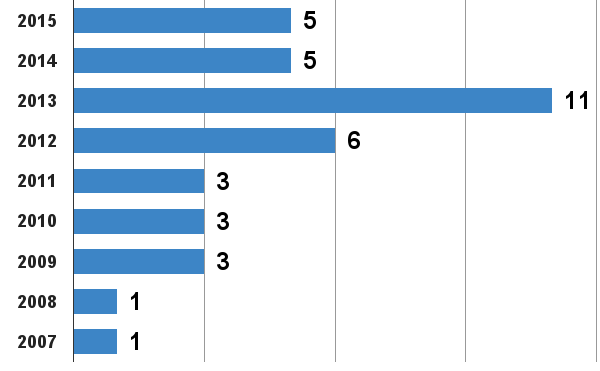
\includegraphics[width=\linewidth]{./fig/survey.png}}
%  \caption{Topic modeling in SE: recent papers since 2007.}
%  \label{fig:survey1}
%\end{figure}



\noindent
Using these datasets, we explore these research questions:  
   
\begin{itemize}


\item \textbf{RQ1}: \textbf{Are the default settings of LDA incorrect?} We will show that using the default settings of LDA for SE data can lead to systematic errors since stability scores start to drop after $n=5$ terms per topic.
    \item \textbf{RQ2}: \textbf{Does LDADE improve the stability scores?} In our work, we will show dramatic improvement in the stability scores with the parameters found automatically by DE. And we also found that the most important parameters which affect cluster stability are $\alpha$ and $\beta$.
    \item \textbf{RQ3}: \textbf{Does LDADE improve the classification F2 accuracy scores?} We will show improvement in the F2 scores with the parameters found automatically by DE. We found that for classification, $k$, number of topics matters the most.
    \item \textbf{RQ4}: \textbf{Do different data sets
      need different configurations to make LDA stable?} We will show that DE finds different ``best'' parameter settings for different data sets. Hence reusing tunings  suggested  by  other  researchers  from other  data  sets are a bad idea.  Instead,  use  automatic  tuning  methods  to find the best tuning parameters for the current data set.
      \item \textbf{RQ5}: \textbf{Using different kinds of LDA or with different implementations, are our findings consistent?} Results were collected across different implementations of LDA (Python+Scikit-Learn, Scala+Spark); across different platforms (Linux, Macintosh) and for different kinds of LDAs (the traditional VEM method, or using Gibbs sampling). Our results found out to be quite consistent and all our above research questions results hold valid in these scenarios as well. Instability is not due to any quirk in the implementation of LDA. Instability is consistent and LDADE can stabilize. 

    \item \textbf{RQ6}: \textbf{Is tuning easy?} We show that, measured
      in the terms of the internal search space of the optimizer,
      tuning LDA is much simpler than standard optimization methods.
    \item \textbf{RQ7}: \textbf{What is the runtime cost of tuning?}
      The advantages of  LDADE come at some cost:
      tuning with DE makes LDA three to five times slower.
      While this is definitely more than not using LDA, this may not be an arduous increase
      given modern cloud computing environments. 
    \item \textbf{RQ8}: \textbf{Should topic modeling be used ``off-the-shelf'' with their default tunings?}
      Based on these findings, our answer to this question is an emphatic ``no''. We can see little reason to use ``off-the-shelf'' LDA for any kind of SE data mining applications.
\end{itemize}

Before proceeding, we found some other important conclusion as to why stability in LDA matters.
Firstly, having mitigated for unstable topics in LDA, the reader may be making conclusions just like from Table~\ref{tbl:run}. And this leading to systematic errors and engineers putting in more effort at the wrong junctions. In a companion paper submitted to IST journal ~\cite{mathews17}
we apply LDADE to 15121 SE papers to find trends in topics between
  1992 to 2016.
That paper reports, what topics are
 becoming more/less prominent; what topics are most frequently accepted to what conferences; which conferences mostly  overlap with other conferences; and what topics most distinguish different
 conferences. Our stable LDADE selected optimal parameters against as selected by Garousi et al~\cite{garousi2016citations}.
 
Secondly, as
witnessed by the central columns of Table~\ref{tbl:survey2},
many prior papers have
commented that the results of a topic modeling analysis can be affected by
tuning the control parameters of LDA.  Yet a repeated pattern in the literature
is that, despite these stated concerns,
researchers rarely take the next step
to find ways to better control tunings. Many researchers did try to find optimal parameter settings using Genetic Algorithms~\cite{panichella2013effectively,lohar2013improving,sun2015msr4sm}. But none of them have considered the most important aspect of LDA which is data input ``order effects''. To the best of our knowledge, apart from this paper, there are no reports in the SE literature of simple reproducible automatic methods that can resolve the problem of unstable topic models. 


Thirdly, while the specifics of this paper are about taming instability in topic modeling,
we also think that this work makes a more general point. To automatically
      adjust the control parameters of a data miner can lead to large improvements in the performance
      of those predictors and that those tunings are different in different data sets. So, it is important to apply automatic tuning as part of the analysis of any new data set. These results suggests that it is time to revisit
      past results to check:
      \bi
    \item
       In the past, just
      how poorly have we been using software analytics
      in the past?
    \item
      And how much better can we improve future results using methods taken from search-based
      software engineering?
      \ei


%% only two authors acknowledged the impact of
%% tunings. In fact  35\% papers in our 57 papers did not adjust the ``off-the-shelf''
%% tunings  of the LDA. Of  the others 65\%, 83\% papers, explored the
%% configurations space with brute force\footnote{u nean a grid search? or a ``engineering judgement''
%%   to set a few param?}. Their was not an effective and faster way
%% of choosing the right set of parameters. Those papers, which accepted the
%% problem of instability in LDA, came to some conclusions which can be found in
%% Table \ref{tb:survey2}. Conclusions of remaining papers are categorized in the
%% following subsections.


%% More generally
%% Wei et al~\cite{fu2016tuning} have shown that one of the simplest \textit{\textbf{multiobjective optimizers (differential evolution}}~\cite{storn1997differential}) works very well for tuning in certain kinds of software analytics. There has been success stories where DE has helped in tuning the parameters~\cite{bazi2014differential, chiha2012tuning}. Prior to this work, our intuition was that tuning would change the behavior of LDA, to some degree. Also, we suspected that tuning would take so long time and be so CPU intensive that the benefits gained would not be worth the effort. We have now seen large instability in 2 data miners, namely, defect predictors and LDA. Results have shown that we can contain the instability to a large extent using DE. So, this makes us wonder Search-Based Software Engineering (SBSE) techniques can help us.

%% Based on answers to these questions, we can surely mitigate the instability of non-deterministic LDA. LDA should not be used with “off-the-shelf” default tunings. Any future paper on LDA should include a tuning study. Tuning needs to be repeated whenever data or goals are changed.

%% Topic Modeling have been used in various spheres of SE. Sun et al reported a survey of LDA's usage to support various SE tasks between 2003 and 2015~\cite{sun2016exploring}. The number of papers published across top major conferences and journals are listed in Table \ref{tab:venues}. The survey in figure \ref{fig: survey} show that there is an increasing concern in this area.


%% \begin{compactitem}
%%     \item Topic modeling is applied in various SE tasks, including source code comprehension, feature location, software defects prediction, developer recommendation, traceability link recovery, re-factoring, software history comprehension, software testing and social software engineering.
%%     \item There are works in Requirements Engineering where it was necessary to analyze the text and come up with the important topics~\cite{asuncion2010software, thomas2014studying, massey2013automated}.
%%     \item People have used topic modeling in prioritizing test cases, \& identifying the importance of test cases~\cite{hemmati2015prioritizing, zhang2015inferring, yang2015predicting}.
%%     \item Increasingly, it has become very important to have automated tools to do a Systematic Literature Review (SLR) ~\cite{tsafnat2014systematic}. We found these papers~\cite{restificar2012inferring,alreview,marshall2013tools} who have used clustering algorithms (topic modeling) to do SLR.
%% \end{compactitem}

%% Since topic modeling has been widely used in various spheres of SE, and it is really important to generate stable topics. Prior Papers who reports LDA may have been severely compromised. This gives all of us the motivation of generating stable topics in software engineering which will make product development faster, cheaper and accurate.

\section{Related Work}

\subsection{Tuning: Important and Ignored}
\label{sect: tuning}

The impact of tuning are well understood in the theoretical machine learning literature~\cite{bergstra2012random}.  When we tune a
data miner, what we are really doing is changing how a learner applies its
heuristics. This means tuned data miners use different heuristics, which means
they ignore different possible models, which means they return different models;
i.e. \textit{how} we learn changes \textit{what} we learn.

Yet issues relating to
tuning are poorly addressed in the software analytics literature.  Fu et al~\cite{fu2016tuning} surveyed hundreds of recent SE papers in the area
of software defect prediction from static code attributes. They found that most SE
  authors do not take steps to explore tunings (rare exception:~\cite{tantithamthavorn2016icse}). For example, Elish et
  al.~\cite{elish2008predicting} compared support vector machines to other data
  miners for the purposes of defect prediction. That paper tested different
  ``off-the-shelf'' data miners on the same data set, without adjusting the
  parameters of each individual learner.  Yet Fu et al
  showed that (a)~finding useful tunings for software defect prediction is remarkably
  easy using DE;  (b)~different data sets require
  different tunings; hence, for software defect prediction,  (c)~tuning is essential for  all
  new data sets.


Accordingly,  we are now engaged in an on-going research project that explores tuning for software analytics.
\begin{itemize}


\item Find some data mining widely used in SE;
\item Check the conclusions of that data miner under different parameter tunings;
\item See if those different tunings significantly change the results of that learner;
\item Look for ways to better manage the exploration of those tunings. \end{itemize}
This
  paper explores these four steps in the context of topic modeling. 


\subsection{Topic Modeling}\label{sect:tm}

Latent Dirichlet Allocation (LDA) is a generative statistical model that allows
sets of observations to be explained by unobserved groups that explain why some
parts of the data are similar. It learns the various distributions (the set of
topics, their associated word probabilities, the topic of each word, and the
particular topic mixture of each document).
What makes topic modeling interesting is that these algorithms scale to very
large text corpuses.  For example, in this paper, we apply LDA to whole of StackOverflow,
as well as to two other large text corpuses in SE.

Figure~\ref{fig:lda} illustrates topic generation from StackOverflow.
To find these words, LDA explores two probability distributions:
\bi
\item $\alpha=P(k|d)$; probability of topic $k$ in  document $d$.
\item $\beta=P(w|k)$; probability of word $w$ in topic $k$; 
\ei
  Initially, $\alpha,\beta$ may be set randomly as follows:
each word in a document was generated by first randomly picking a topic (from
the document’s distribution of topics) and then randomly picking a word (from
the topic’s distribution of words). Successive iterations of the algorithm 
count the implications of prior sampling which, in turn,  incrementally updates $\alpha,\beta$.

Binkley et al~\cite{binkley2014understanding} performed an extensive study and found that apart from $\alpha,\beta$, the other parameters that define LDA
are:
\bi
\item $k$ = number of topics;
\item $b$ = number of burn-in iterations;
\item $si$ = the sampling interval
\ei

But finally Binkley et al, with all the many researchers found the only important parameters that matters the most are $k$, $\alpha$, $\beta$. Even our results showed the same. Binkley et al didn't provide any automatic methods to find these settings. They haven't even covered  the possibility of input ordering of data samples.

\begin{figure}[!t]
\scriptsize
\begin{center}
\begin{tabular}{c|c|c|c|c}
 
        \begin{tabular}[c]{@{}c@{}}Topic: String\\ Manipulation\end{tabular}    &\begin{tabular}[c]{@{}c@{}}Topic:\\ Function\end{tabular}    &\begin{tabular}[c]{@{}c@{}} Topic: OO \\Programming\end{tabular} &\begin{tabular}[c]{@{}c@{}}Topic: UI \\Development\end{tabular}&\begin{tabular}[c]{@{}c@{}}Topic: File \\Operation\end{tabular} \\\hline
string&function& class& control&file \\
charact&paramet& method& view&directori\\
encod&pass& object& event&path\\
format&return& call& button&folder\\
convert&argument& interfac& click&creat\\\hline
\end{tabular}
\end{center}
\caption{Example (from~\cite{barua2014developers}) %grus15
of generating topics from StackOverflow. For each topic, we show just the five most heavily
  weighted words.}\label{fig:lda}

\end{figure}

%\begin{center}
%\begin{tabular}{c|c|c|c}
 
%           Topic 0 &Topic 1 &Topic 2 &Topic 3\\\hline
%Java& R& HBase &regression\\
%Big Data& statistics& Postgres& libsvm\\
%Hadoop& Python& MongoDB& scikit-learn\\
%deep learning& probability& Cassandra& machine learning\\
%artificial intelligence& pandas& NoSQL& neural networks\\\hline
%\end{tabular}
%\end{center}
%\caption{Example (from~\cite{oliveto2010equivalence}) %grus15
%of generating topics (at bottom) from the
%  keywords from 15 document
%  (shown at top). For each topic, we show just the five most heavily
%  weighted words.}\label{fig:lda}
%\end{figure}


\subsection{About Order Effects}

\noindent
This paper uses tuning to fix ``order effects'' in topic modeling. Langley~\cite{GENNARI198911} defines such effects as follows:
\begin{quote}
{\em A learner $L$ exhibits an order effect on a training set  $T$ if there exist
two or more orders of $T$ for which $L$ produces different knowledge structures.}
\end{quote}
Many learners exhibit order effects: e.g. certain incremental clustering algorithms generate different
clusters, depending on the order with which they explore the data~\cite{GENNARI198911}.
Hence, some algorithms survey the space of possible models across numerous
random divisions of the data (e.g. Random Forests~\cite{Breiman2001}).

From the description offered above in \S\ref{sect:tm},
we can see (a)~how topic modeling might be susceptible to order effects and (b)~how such order
effects might be tamed:
\bi
\item
  In the above description, $k$, $\alpha,\beta$ are initialized at random
then updated via an incremental re-sampling process. Such incremental updates are prone to order effects.
\item
  One technique to reduce the effect of different data orderings is to initialize, $k$, $\alpha,\beta$ to some
  large value. The trick when applying this technique is that different data sets will requiring different
  initializations; i.e. the tuning process will have to be repeated for each new data set.
\ei
  
%%   Apart fro order effects, another reason for instability within LDA are the random choices
%%   made within Another reason for ins  
%% \subsection{About Topic Modeling and LDA}


%% Note that if LDA considers the training data $T$ in another ordering, other topics might be discovered.
%% Later in this article, when we explore  {\bf RQ1}, we will see that for SE data that this instability can be substantial.


%% %YYY need 5 lines on VEM and GS

%% Under the hood, LDA uses Bayesian inference to represent and update
%% $P_1,P_2$ which, in turn my use  alternative inference techniques like Gibbs
%% sampling~\cite{wei2006lda, griffiths2004finding} or variational expectation
%% maximization (VEM)~\cite{minka2002expectation}. These techniques in LDA try to
%% maximize the resulting lower bound on the log
%% likelihood~\cite{blei2003latent}. Note that the expected complete log likelihood of the
%% data have many local maximas, which leads to different distributions and in turn
%% leads to instability in the output.

%% %% The distributions which are found with the
%% %% help of LDA, resulting from the same dataset with the same vocabulary and model
%% %% parameters, any differences between them are entirely due to the randomness in
%% %% inference techniques~\cite{koltcov2014latent}. This randomness affects word and
%% %% document ratios. There is a problem of finding the optimal number of clusters,
%% %% but different configuration parameters may lead us to the stable topics.

%% %% The topics learned by LDA sometimes are difficult to interpret by end
%% %% users~\cite{yang2015improving, panichella2013effectively}. We want topics to be
%% %% finer grained (more number of topics) or coarse grained (less number of topics)
%% %% according to the use case. Rationality about the topics instability is important
%% %% if an industry is using topic modeling in all their use
%% %% cases~\cite{lau2014machine, o2015analysis}. We do not want vaguely defined
%% %% topics.

%% Recent work with online learning LDA~\cite{hoffman2010online} propose algorithms
%% that, empirically,
%% converge quickly to its final $P_1,P_2$ values.  %YYY do i have to that rightfaster than batch collapsed Gibbs
%% The external validity section of this paper will test if these fast convergence methods remove the instability problem.
%% %YY is this the gibbs stuff?

%We observed that this is just not happening with only particular programming language or particular library. This instability is happening irrespective of the tools in which LDA has been implemented. Some of the papers mentioned using GibbsLDA++ written in C++ and they observed the same instability~\cite{lukins2008source, tian2009using, guzman2014users}. Some papers mentioned about using Python implementation of LDA and observed the same instability~\cite{guzman2014users}. LDA implemented in JAVA language produced the same incoherent topics~\cite{martin2015app, hindle2011automated}. And, we observed this problem is in the Scikit-Learn version of LDA, implemented in Python, as well as Spark Mllib library.



\subsection{WorkArounds for LDA Instability Problem}
\label{sect: solutions}
%YYY
In order to understand how other researchers have explored LDA instability,
in April 2016, we searched scholar.google.com for the conjunction of ``lda'' and ``topics'' or ``stable'' or
``unstable'' or ``coherence''. Since 2012, there are  189 such papers, 57
of which are related to software engineering results. Table \ref{tbl:survey2} gives a broad discussion on these papers. In short, of those papers:
\bi
\item 29
mention instability in LDA. %(more details can
%be found at \href{https://goo.gl/Bpc6Vb}{\textit{https://goo.gl/Bpc6Vb}}).
\item Of those 29, despite mentioning stability problems,
  10 papers used LDA's ``off-the-shelf'' parameters;
  \item The  other papers used some combination of manual adjustment or some
under-explained limited exploration of tunings based on ``engineering judgment''
(i.e. some settings guided by the insights of the researchers).
\item
Only 4 of the authors acknowledge that tuning might have a large impact
on the results.
\ei
Apart from tuning, there are several other workarounds explored in the literature
in order to handle LDA instability. Overall, there was little systematic exploration of tuning and LDA in the SE literature.
Instead, researchers relied on other methods that are less suited to automatic reproduction of prior results.

In the literature, researchers~\cite{maskeri2008mining, martin2015app, guzman2014users}
    manually accessed the topics and then used for further experiments. Some
    made use of Amazon Mechanical Turk to create gold-standard coherence
    judgements~\cite{lau2014machine}. All these solutions are related to results
    stability rather than model stability.
    Note that this workaround takes extensive manual effort and time.

    
    Another approach to tame LDA instability
    is to incorporate
    user knowledge into the corpus. For example,
    SC-LDA~\cite{yang2015improving} can
    handle different kinds of knowledge such as word correlation,
    document correlation, document label and so on. Using such user
    knowledge, while certainly valuable, is somewhat subjective.
    Hence, for reasons of reproducibility, we prefer fully
    automated methods.

%UYY need to sort this
Some researchers~\cite{panichella2013effectively, lohar2013improving, sun2015msr4sm}
used Genetic Algorithm (GA) to tune the parameters-- but for different
purposes than LDADE. Panichella et al~\cite{panichella2013effectively} used GAs to explore parameters. This method is quite time consuming than using a simple multiobjective optimizer like differential evolution~\cite{storn1997differential}. They have not even explored the problem of input ordering of data samples. But the gain from their studies was that finding good optimal settings of LDA could give us larger improvement in their results.

Finally, other researchers explore
some limited manual parameter tuning for LDA
(e.g. experiment with one parameter: cluster size)~\cite{galvis2013analysis, tian2009using}
achieved higher stability by just increasing the number of cluster size.
Note that the automatic tuning methods explored by this paper can
explore multiple parameters. Further, our analysis is repeatable.

\section{Methods}
\label{sect:evaluation}
This section describes our evaluation methods for measuring instability as well as the optimization
methods used to reduce that instability.


\begin{table}[!t]
\begin{center}
\begin{tabular}{c|r|r}
  \begin{tabular}{cc@{}c@{}}
    \multicolumn{2}{c}{\textbf{~}}
  \end{tabular}
  & \multicolumn{2}{c}{\textbf  Size} \\
    \cline{2-3}
         & \textbf{Before} & \textbf{After}\\ 
  \textbf{Data set}      & \textbf{Preprocessing} & \textbf{Preprocessing}\\ 
        \hline
        PitsA & 1.2 MB & 292 KB \\ 
        \hline
        PitsB & 704 KB & 188 KB \\
        \hline
        PitsC & 143 KB & 37 KB \\ 
        \hline
        PitsD & 107 KB & 26 KB \\ 
        \hline
        PitsE & 650 KB & 216 KB \\
        \hline
        PitsF & 549 KB & 217 KB \\ 
        \hline
        Citemap & 8.6 MB & 3.7 MB \\ 
        \hline
        StackOverflow & 7 GB & 589 MB \\ 
\end{tabular}
\end{center}
\caption{Statistics on our datasets. PitsA, PitsB, etc refer to the issues
from six different NASA projects.}
\label{tbl:dataset}
\end{table}
\begin{figure*}[!t]
  \begin{center}
    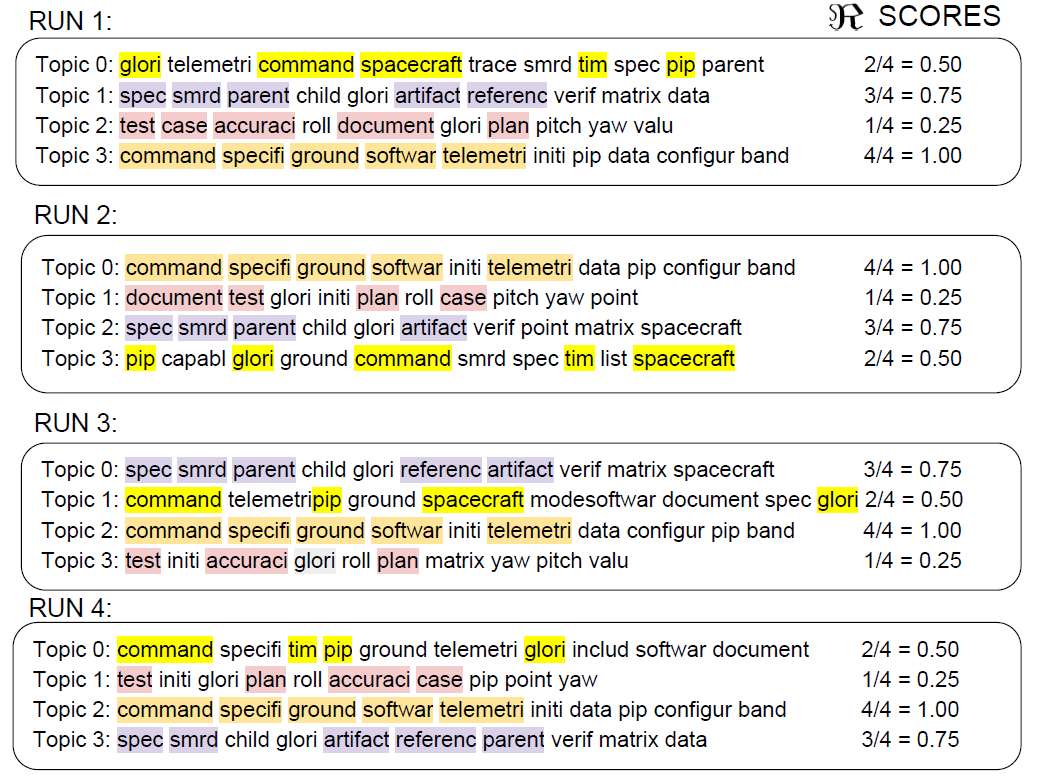
\includegraphics[width=13cm]{./fig/jaccard.png}
    \end{center}
  \caption{Example of topics overlap off size $n=5$ across multiple runs.}
  \label{fig:jaccard}
\end{figure*}


\subsection{Data Sets}
To answer our research questions, and to enable reproducibility of our results,
we use three open source datasets summarized in Table~\ref{tbl:dataset} and described
below.

\textbf{PITS} is a text mining data set generated from NASA software project
and issue tracking system (PITS) reports~\cite{menzies2008improving,
  menzies2008automated}. This text discusses
bugs and changes found in big reports and  review patches.
Such issues are used
to manage quality assurance, to support communication
between developers. Topic modeling in PITS can be used
to identify the top topics which can
identify each severity separately. The dataset can be downloaded from the
PROMISE
repository~\cite{promiserepo}. Note that, this data comes from six different
NASA projects, which we label as PitsA, PitsB, etc.
    
 \textbf{StackOverflow} is the flagship site of the Stack Exchange Network which
 features questions and answers on a wide range of topics in computer
 programming.
Topic modeling on StackOverflow is useful for finding patterns in programmer knowledge.
 This data can be downloaded online\footnote{http://tiny.cc/SOProcess}. 
    
  \textbf{Citemap} contains titles and abstracts of 15121 papers from a
 database of 11 senior software engineering conferences from 1992-2016. This data was
 obtained in the form of an SQL dump from the work of Vasilescu et
 al.~\cite{vasilescu2013historical}.  This dataset is available on-line\footnote{https://github.com/ai-se/citemap/blob/master/citemap.csv}.

  For this study, all  datasets were preprocessed using the usual text mining filters~\cite{feldman2006j}:
\bi
\item
  Stop words removal using NLTK toolkit\footnote{http://www.nltk.org/book/ch02.html}~\cite{bird2006nltk} : ignore very common short words such as  ``and'' or ``the''.
\item
  Porter's stemming filter~\cite{Porter1980}: delete uninformative word endings; e.g. after stemming, all the following words would be rewritten
  to ``connect'': ``connection'', ``connections'',
``connective'',          
``connected'',
  ``connecting''.
\item
  Tf-idf feature selection: focus on the 5\% of words that occur frequently,
  but only in small numbers of documents. If a word occurs $w$ times
  and is found in $d$ documents  and there
  are $W,D$ total number of words and documents respectively, then tf-idf is scored
  as follows:
  \[
  \mathit{tfidf}(w,d)=   \frac{w}{W} *\log{\frac{D}{d}}\]
  \ei

  Table~\ref{tbl:dataset} shows the sizes of our data before and after pre-processing.
  These datasets are of different sizes and so are processed using different tools:
  \bi
\item PITS and Citemap is small enough to process on a single (four core) desktop machine
  using Scikit-Learn~\cite{pedregosa2011scikit} and Python.
  \item StackOverflow is so large (7GB) that its  processing requires extra hardware support.
 This study used a Spark and Mllib on a cluster of 45 nodes to
 reduce the runtime.
 \ei
  




\subsection{Similarity Scoring}
%YY this apra makes no sense
%% To evaluate the topics coherence or the cluster stability using LDA, there has
%% been number of evaluation measures proposed. There is a direct approach, by
%% asking people about topics, and an indirect approach by evaluating
%% \textit{pointwise mutual information (PMI)}~\cite{lau2014machine, o2015analysis}
%% between the topic words. PMI being an automatic method, we are not sure of exact
%% details of it which made us to not use this measure. We could not use direct
%% approach, due to resource limitation to ask an expert for the type of datasets
%% we used.
To evaluate topics coherence in LDA, there is a direct approach, by asking people about topics, and an indirect approach by evaluating \textit{pointwise mutual information (PMI)}~\cite{lau2014machine, o2015analysis} between the topic words. We could not use any of these criteria, as it requires experts to have domain knowledge. \textit{Perplexity} is  the inverse of the geometric mean per-word likelihood. The smaller the perplexity, the better (less uniform) is the LDA model. The usual trend is that as the value of perplexity drops, the number of topics should grow~\cite{koltcov2014latent}. Researchers caution that the value of perplexity doesn't remain constant with different topic size and with dictionary sizes~\cite{koltcov2014latent, zhao2015heuristic}. A lot depend on the code implementation of perplexity and the type of datasets used. Since, we are using different implementations of LDA across different platforms on various datasets, we are not using perplexity as evaluation measure.

Another approach researchers have used is \textit{Jaccard Similarity}~\cite{o2015analysis, galvis2013analysis}. We define our measure similar to it. For this work, we assess topic model stability via the {\em median number overlaps of size $n$ words $\mathit{(size\_of\_topic)}$}, which we denote  $\Re_n$.

%XXX  The magical number seven plus or minus two: some limits on our capacity for processing information.
%by: G. A. MILLER
%Psychological review, Vol. 63, No. 2. (March 1956), pp. 81-97  Key: citeulike:1089248
 


For this measurement, we first determine the maximum size of topics we will study. For that purpose,
we will study the case of $n \le 9$ (we use 9 as our maximum size since the cognitive
science literature tells us that $7\pm 2$ is a useful upper size for artifacts to be browsed by humans~\cite{miller1956magical}).


Next, for $1 \le n \le 9$, we will calculate the median size of the overlap,
computed as follows:
\bi
\item Let one {\em run} of our rig shuffle the order of the training data, then builds topic models using the data;
  \item $m$ runs of our rig executes $m$ copies of one run, each time using a different random number seed,
\item We say topics are stable,
when there are $x$ occurrences of  $n$ terms appearing in all the topics seen in the $m$ runs.
\ei


For example, consider the topics shown in Figure~\ref{fig:jaccard}. These are generated via four {\em runs} of our system. In this hypothetical example, we will assume that the runs of
 Figure~\ref{fig:jaccard} were generated by an LDA suffering from topic instability.
For $n=5$, we note that Topic~0 of run1 scores $\frac{2}{4}=0.5$ since it shares 5 words with topics in only two out of four runs.
Repeating that calculation for the other run1 topics shows that:
\bi
\item Topic~1 of run1 scores $\frac{3}{4}=0.75$;
\item Topic~2 or run1 scores $\frac{1}{4}=0.25$;
\item Topic~3 of run1 scores $\frac{4}{4}=1$.
  \ei
  From this information, we can calculate
  $\Re_5$  (the
  {\em median number overlaps of size $n=5$ words}) as:
  \[
   \mathit{median}(0.5, 0.75, 0.25, 1) =0.625\]
  %YYY need an example of Fig5 here using the data of Figure4.
  Figure~\ref{fig:alln}
  shows the $\Re_n$ scores of 
  Figure~\ref{fig:jaccard} for $1 \le n \le 9$.  From this figure, we can see LDA topic instability
  since
  any report of the contents of a topic that uses more than three words per topic would be unreliable.

  \begin{figure}[!h]
  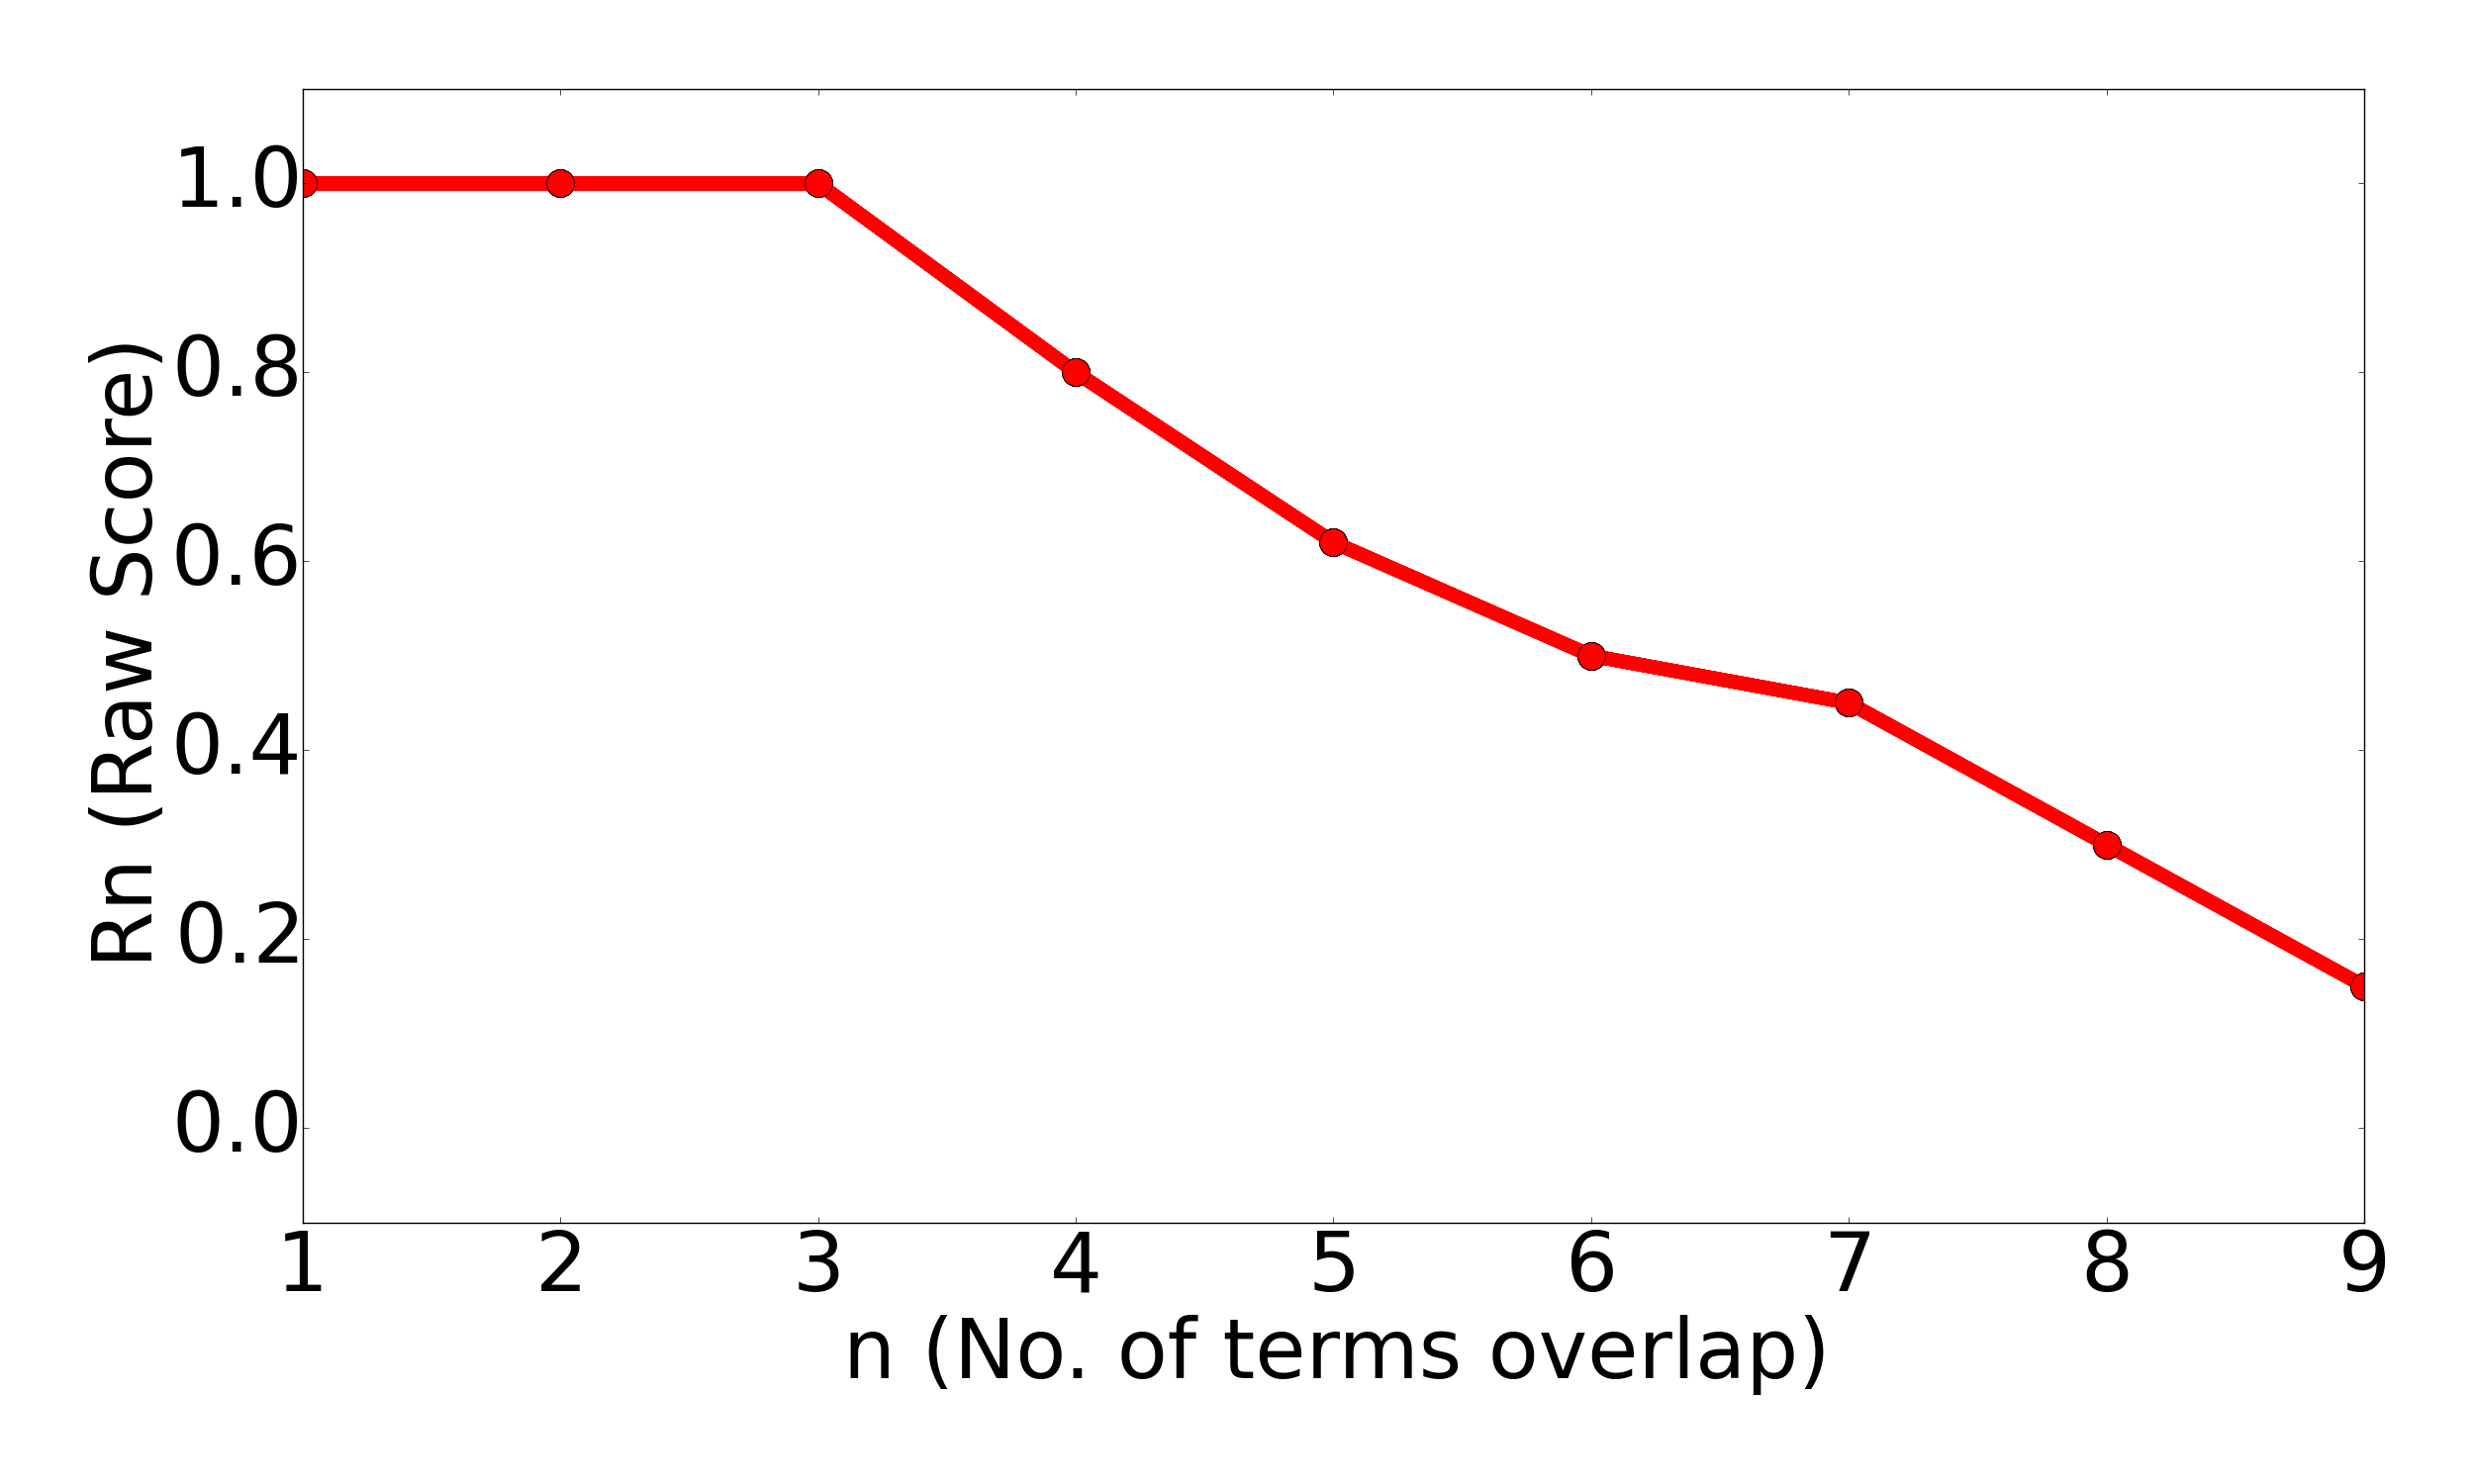
\includegraphics[width=\linewidth]{./fig/alln.png}
  \caption{$\Re_n$ scores of 
  Figure~\ref{fig:jaccard} for $1 \le n \le 9$}
  \label{fig:alln}
\end{figure}

 For the following analysis,
 %YYY do our graphs really use this terminology?
we distinguish between the \textbf{\textit{Raw  score}} and the \textbf{\textit{Delta  score}}:
 \bi
\item The two \textbf{\textit{Raw  scores}} are the $\Re_n$ median similarity scores seen {\em before} and {\em after} tuning LDA;
\item The \textbf{\textit{Delta score}} is the difference between the two
  \textbf{\textit{Raw scores}} (after tuning - before tuning).  \ei 
  The pseudocode for these calculations
  is shown in Algorithm 1 with the default set of parameters. In the following
  description, superscript numbers denote lines in the pseudocode. The data ordering is
  shuffled every time LDA is run$^{5}$. Data is in the form of term frequency
  scores of each word per document. Shuffling is done in order to induce maximum
  variance among the ordering of data with  different runs of LDA. Topics$^{6}$ are a list of lists which
  contains topics from all the different runs. A stability score is evaluated on
  every 10 runs (Fixed), and this process is continued 10 (Fixed) times. At the end, the median
  score is selected as the untuned raw score ($\Re_n$ ) $^{3-11}$. Hence, the runtimes comes from $10 * 10$ evaluations of untuned experiment.

\makeatletter
\algrenewcommand\ALG@beginalgorithmic{\footnotesize}
\algrenewcommand\algorithmiccomment[2][\normalsize]{{#1\hfill\(\triangleright\) #2}}
\makeatother
\renewcommand{\algorithmicrequire}{\textbf{Input:}}
\renewcommand{\algorithmicensure}{\textbf{Output:}}
\begin{algorithm}
    %\scriptsize
    %\label{algo: untuned}
    
    \begin{algorithmic}[1]
    %\label{algo: untuned}
    \Require $Data$, $n$, $k$, $\alpha$, $\beta$ (Defaults) 
    \Ensure $Raw\_Score$    
    \Function{ldascore}{ $n$, $Data$}
        \State $Score \leftarrow \emptyset$
        \For{$j = 0$ to 10}
            \For{$i = 0$ to 10}
                \State $data \leftarrow$ \textbf{shuffle}($Data$)
                \State $Topics$.add(lda($k,\alpha,\beta$ ))
            \EndFor
            \State $Score$.add($Overlap$(Topics, $n$, $l[0]$))
        \EndFor
        \State $Raw\_Score \leftarrow $ median(Score)
        \State \textbf{return} $Raw\_Score$
    \EndFunction
    %\medskip
    \caption{Pseudocode for untuned LDA with Default Parameters}
    \end{algorithmic}
\end{algorithm}

%YYY: who first proposed LDA... need a referece first time we mention if
\subsection{Tuning Topic Modeling with LDADE}
\label{sect: tuning}
LDADE is a combination of topic modeling (with LDA) and an optimizer (differential evolution, or DE) that adjusts
the parameters of LDA in order to optimize (i.e. maximize) similarity scores.

We choose to use DE after a literature search on search-based SE methods.
The literature mentions many optimizers: simulated
annealing~\cite{feather2002converging, menzies2007business}; various genetic
algorithms~\cite{goldberg1979complexity} augmented by techniques such as
DE (differential evolution~\cite{storn1997differential}), tabu search and scatter
search~\cite{glover1986general, beausoleil2006moss, molina2007sspmo,nebro2008abyss}; particle swarm optimization~\cite{pan2008particle}; numerous
decomposition approaches that use heuristics to decompose the total space into
small problems, then apply a response surface methods~\cite{krall2015gale, zuluaga2013active}.
Of these, we use DE for two reasons. Firstly, it has proved useful in prior SE tuning
studies~\cite{wei2006lda}. Secondly,   our reading of the current literature is
that there are many advocates for differential evolution.

%\newpage
LDADE  adjusts the parameters of
Table~\ref{tb:tuned}. Most of these parameters were explained above. Apart from them, there are 2 different kinds of LDA implementations as well and they are:
\bi
\item VEM is the deterministic {\em variational EM} method that computes $\alpha,\beta$ via
  expectation maximization~\cite{minka2002expectation}.
\item Gibbs sampling~\cite{wei2006lda, griffiths2004finding} is a Markov Chain Monte Carlo algorithm, which is an approximate stochastic process for computing and updating $\alpha,\beta$.
  Topic modeling researchers in SE have argued that Gibbs leads to stabler models~\cite{layman16a,layman2016topic} (a claim which we test, below).
  \ei

We manually run with these other inference techniques according to different implementations across different platforms. We need to make sure that these instabilities do not hold for just 1 inference technique, or 1 implementation or on 1 platform.

\begin{table}[!htbp]
    \begin{center}
{\scriptsize
\begin{tabular}{|l|l|l|p{3.5cm}|}
        \hline 
        \textbf{Parameters} & \textbf{Defaults} & \textbf{Tuning Range} & \textbf{Description}\\
        \hline
        $k$ & 10 & [10,100] & Number of topics or cluster size \\ 
        \hline
       $\alpha$ & None & [0,1] & Prior of document topic distribution. This is called alpha \\ 
        \hline
        $\beta$ & None & [0,1] & Prior of topic word distribution. This is called  beta \\

        \hline
\end{tabular}
}
\end{center}
\caption{List of parameters tuned by this paper}
\label{tb:tuned}
\end{table}

Algorithm 2 shows LDADE's version of DE.  DE evolves a \textit{NewGeneration} of
candidates from a current Population.   Each candidate solution in the Population is a pair of
(Tunings, Scores). Tunings are selected from Table \ref{tb:tuned} and Scores
come similarly from Algorithm 1$^{3-11}$. Note that there is not any outer loop$^{3}$: in Algorithm 2, LDA is only run as 1 rig$^{11 \& 12}$. Here, the runtimes comes from $\mathit{iter} * np * 10$ evaluations of tuned experiment.

The main loop of DE$^{9}$ runs over the \textit{Population}, replacing old items with new Candidates (if new candidate is better).
DE generates \textit{new Candidates} via 
extrapolating$^{23}$ between current solutions in the frontier. Three solutions a, b, c\textit{} are
selected at random. For each tuning parameter i, at some probability \textit{cr}, we
replace the old tuning $x_i$ with $y_i$. For booleans, we use $y_i = x_i$ (see
line 31). For numerics, $y_i = a_i + f \times (b_i - c_i)$ where f is a
parameter controlling crossover. The trim function$^{33}$ limits the new value
to the legal range min..max of that parameter.

The loop invariant of DE is that, after the zero-th iteration$^7$, the \textit{Population}
contains examples that are better than at least one other candidate.
As the looping progresses, the \textit{Population} is full of increasingly more valuable solutions
which, in turn, also improves the candidates, which are Extrapolated from the Population.
Hence, Vesterstrom et al~\cite{vesterstrom2004comparative} found DE to be
competitive with particle swarm optimization and other GAs.

Note that DEs have been
applied before for parameter tuning (e.g. see~\cite{panichella2013effectively, lohar2013improving, sun2015msr4sm,omran2005differential,chiha2012tuning, fu2016tuning} ) but this is the first time they have been
applied to tune LDA to increase stability.

\section{Experimentation}

In this section,
 any result from the smaller data sets (Pits and Citemap) come
from Python implementation based on Scikit-Learn running on a single 4-core machine.
Also,
  any results from the larger data (StackOverflow) comes from a Scala implementation
  based on Mllib~\cite{meng2016mllib} running on a 45 node Spark system (8 cores per node).
  
  Note that, for the RQ3, there are some intricate details with classification results. After tuning and finding the optimal `K', we trained a Linear Kernel SVM classifier using document topic distributions as features just like used by Blei et al~\cite{blei2003latent}.

\renewcommand{\algorithmicrequire}{\textbf{Input:}}
\renewcommand{\algorithmicensure}{\textbf{Output:}}
\begin{algorithm}
  
    \begin{algorithmic}[1]
    \Require np$=10$, f$=0.7$, cr$=0.3$, iter$=3$, Goal $\in$ Finding maximum score
    \Ensure $Raw\_Score, final\_generation$
    \Function{DE}{$np,f,cr,iter, Goal$}
        \State  $Cur\_Gen \leftarrow \emptyset$
        \State $Population \leftarrow $InitializePopulation(np)
        \For{$i = 0$ to $np-1$}
            \State $Cur\_Gen$.add($Population$[i],ldascore($Population$[i],$n$,$Data$)
        \EndFor
        \For{$i = 0$ to $iter$}
            \State $NewGeneration \leftarrow \emptyset$
            \For{$j = 0$ to $np-1$}
                \State $S_i \leftarrow $Extrapolate($Population$[j],Population,cr,f,np)
                \If{ldascore($S_i$) $\geq$ $Cur\_Gen$[j][1]}
                    \State $NewGeneration$.add($S_i$,ldascore($S_i$,$n$, $Data$))
                \Else
                    \State $NewGeneration$.add($Cur\_Gen$[j])
                \EndIf
            
            \EndFor
            \State  $Cur\_Gen \leftarrow NewGeneration$
        \EndFor
        \State $Raw\_Score \leftarrow$ GetBestSolution($Cur\_Gen$)
        \State  $final\_generation \leftarrow Cur\_Gen$
        \State \textbf{return} $Raw\_Score, final\_generation$
    \EndFunction

    \Function{Extrapolate}{$old, pop, cr, f,np$}
        \State $a,b,c \leftarrow threeOthers$(pop, old)
        \State $newf \leftarrow \emptyset$
        \For{$i = 0$ to $np-1$}
            \If{$cr \leq$ random()}
                \State $newf$.add($old[i]$)
            \Else
                \If{typeof($old$[i])$ ==$ bool then}
                    \State $newf$.add(not $old[i]$)
                \Else 
                    \State $newf$.add(trim(i,($a$[i]+$f\ast$($b$[i] $-$ $c$[i]))))
                \EndIf
            \EndIf
        \EndFor
        \State \textbf{return} $newf$ 
    \EndFunction
    \caption{Pseudocode for DE with a constant number of iterations}
    \end{algorithmic}
\end{algorithm}

\begin{figure*}[!htbp]
    \centering
    \begin{minipage}{.51\textwidth}
        \begin{center}
        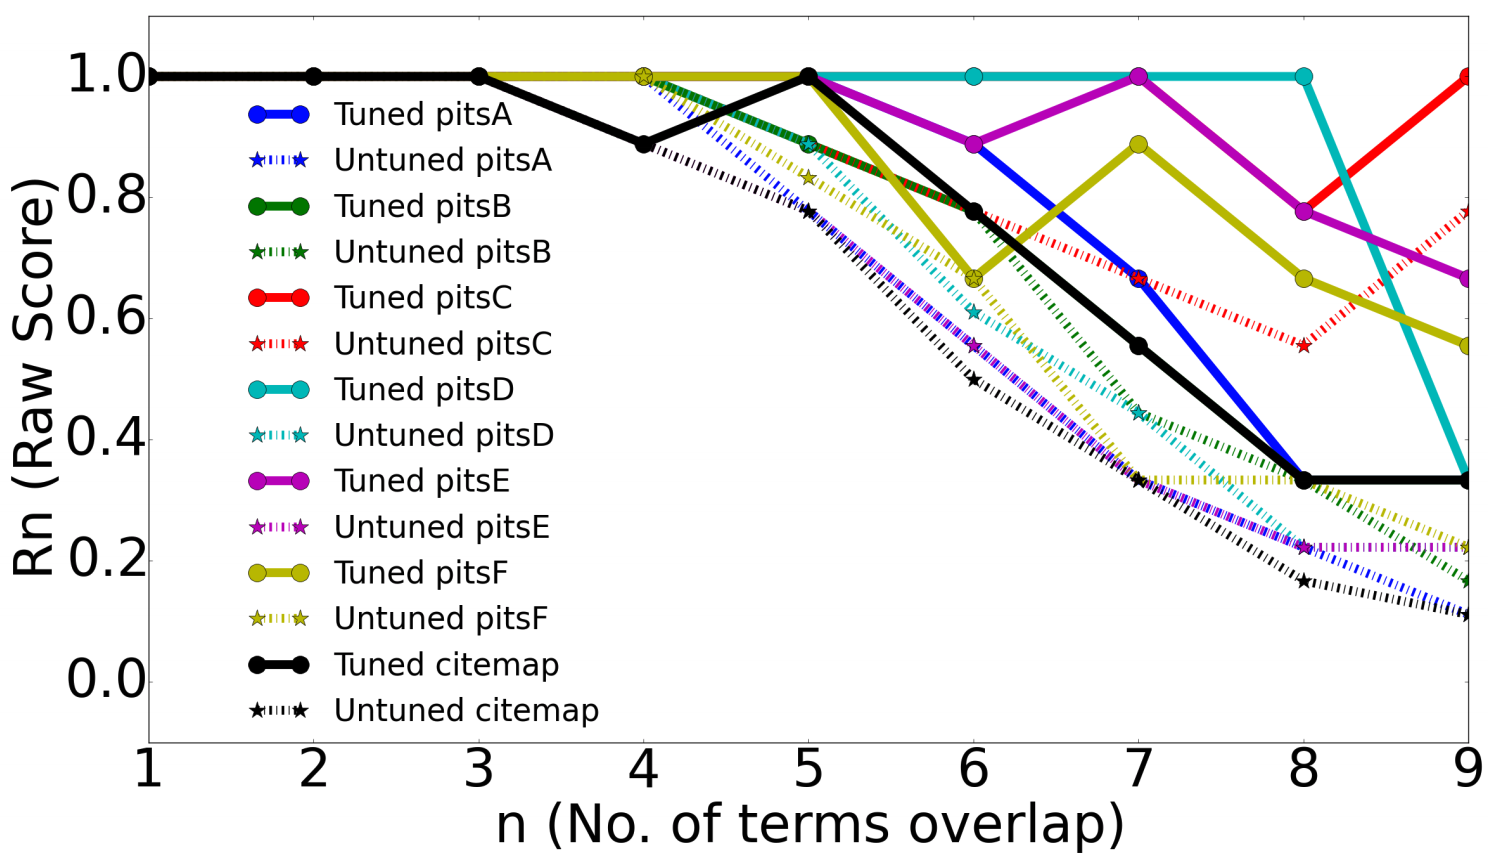
\includegraphics[width=\linewidth]{./fig/raw_graph.png}
  {\bf Figure~\ref{fig:delta}a:}  {\em After} tuning: uses parameters learned by DE.
  \end{center}
    \end{minipage}%
    \begin{minipage}{.5\textwidth}
        \begin{center}
        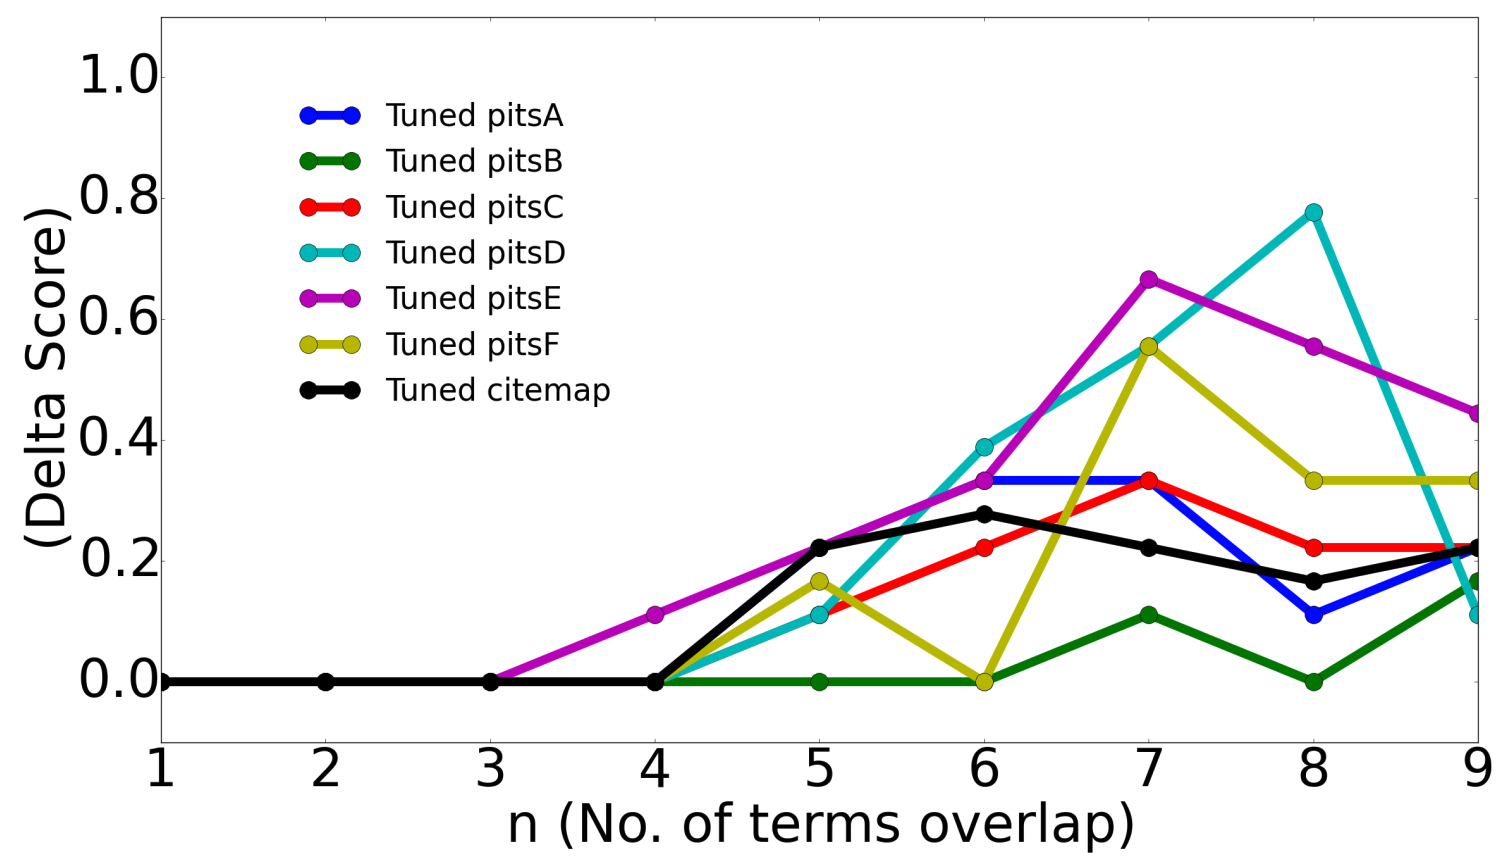
\includegraphics[width=\linewidth]{./fig/tuned_delta_vem.png}
  {\bf Figure~\ref{fig:delta}b:}  {\em Delta = After - Before}.
  \end{center}
    \end{minipage}
    \caption{{\bf RQ1, RQ2} stability results over ten repeated runs. In these figures, {\em larger} numbers
    are {\em better}.}\label{fig:delta}
\end{figure*}

\subsection{\textbf{RQ1: Are the default settings of LDA correct?}}


This first research question checks the core premise of this article-- that changes
in the order of training data dramatically affects the topics learned via LDA.
Note that if this is {\em not true}, then there would be no value-added to this paper.


Figure~\ref{fig:delta11}   plots $n$ vs $\Re_n$ for untuned  LDA.
Note that the  stability collapses the most after $n=5$ words. This means
  that any report of LDA topics that uses more than five words per topic will
  be changed, just by changing the order of the inputs. This is a significant result
  since the standard advice in the LDA papers~\cite{panichella2013effectively, lukins2010bug}
  is to report the top 10 words per topic. As shown in Figure~\ref{fig:delta}a, it would
  be rare that any such 10 word topic would be found across multiple runs.
  
\begin{lesson}
  Using the default settings of LDA for SE data can lead to systematic errors due to topic
  modeling instability. 
\end{lesson}

\begin{figure}[!htbp]
  \begin{center}
    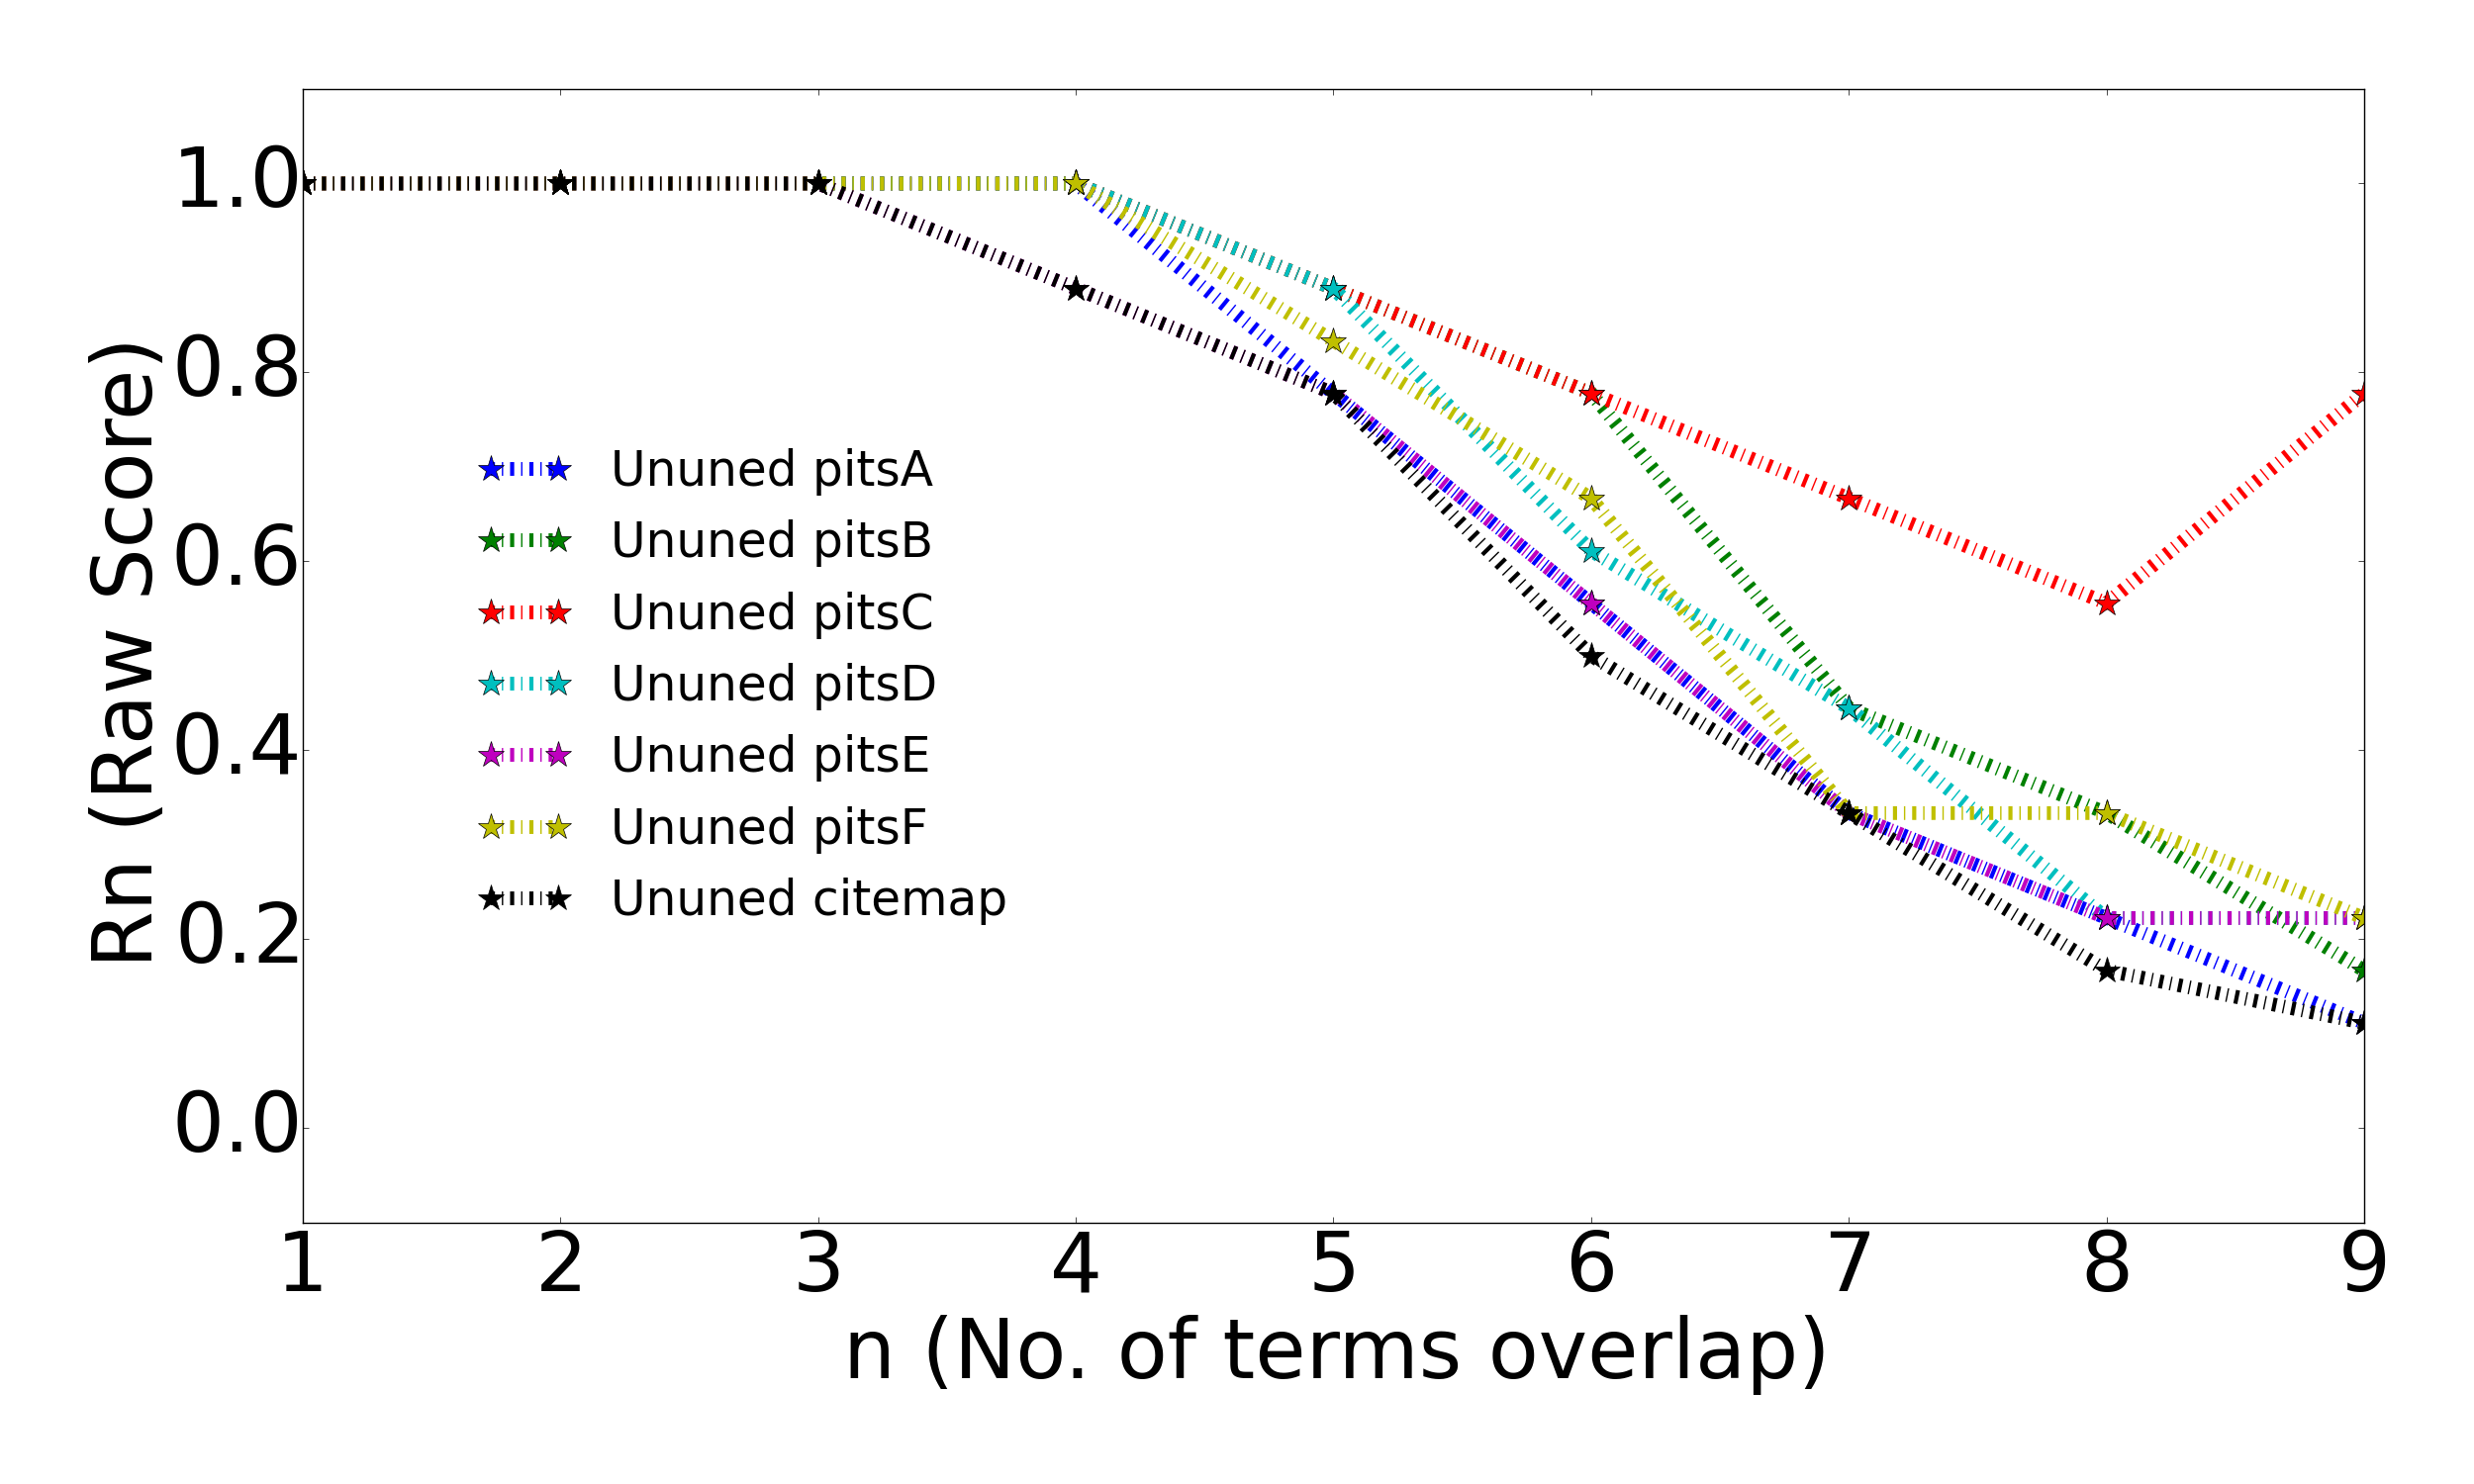
\includegraphics[width=\linewidth]{./fig/Vem_untuned.png}
    \end{center}
  \caption{{\em Before} tuning: uses LDA's default parameters}\label{fig:delta11}  
\end{figure}


\subsection{\textbf{RQ2: Does tuning improve the stability scores of LDA?}}

 Figure~\ref{fig:delta}a and Figure~\ref{fig:delta}b shows the stability improvement
 generated by tuning.
   Tuning never
  has any negative effect (reduces stability) and often has a large positive effect--
  particular  after 5 terms overlap.
   The largest improvement  we
   was  in PitsD dataset which for up to 8 terms overlap was 100\% (i.e. was always
   found in all runs).
   Overall, after reporting topics of up to 7 words, in the majority case (66\%),
  those topics can be found in models generated using different input orderings.
  Accordingly, our answer to {\bf RQ2} is:

\begin{lesson}
For stable clusters, tuning is strongly recommended for future LDA studies. $\alpha$ and $\beta$ matters the most for getting good clusters.
\end{lesson}

\subsection{\textbf{RQ3:Does LDADE improve the classification F2 accuracy scores?}} 

We studied some other StackExchange websites data dump for classification results which were generated by Krishna et al \cite{krishna2016bigse}. These datasets are categorized into binary labels saying which documents are relevant and non relevant. Here goal of our DE was still to maximize the $\Re_n$ score. It shouldn't be confused with maximizing some other accuracy goals. After finding the optimal `K', we trained a Linear Kernel SVM classifier using document topic distributions just like used by Blei et al~\cite{blei2003latent}.

In Figure \ref{fig:class}, x-axis represents different datasets as generated. Y-axis represents the F2 scores which weigh recall higher than precision~\cite{powers2011evaluation}. One legend called as ``untuned'' basically uses default parameters with $k=10$. Other legends in the graph shows tuning of $k$ for 20, 40, 80, 200 by keeping $\alpha$ and $\beta$ fixed. There is about 20\% minimum improvement than the untuned results.

\begin{figure*}[!htbp]
    \centering
    \begin{minipage}{.33\textwidth}
        \captionsetup{justification=centering,singlelinecheck=off}
        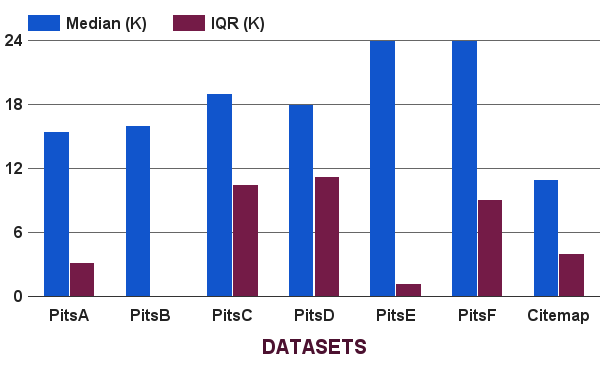
\includegraphics[width=\linewidth]{./fig/Parameters_variation_k.png}
        \caption{Datasets vs Parameter (k) variation}
        \label{RQ3:k}
    \end{minipage}%
    \begin{minipage}{.33\textwidth}
        \captionsetup{labelsep=space,justification=centering,singlelinecheck=off}
        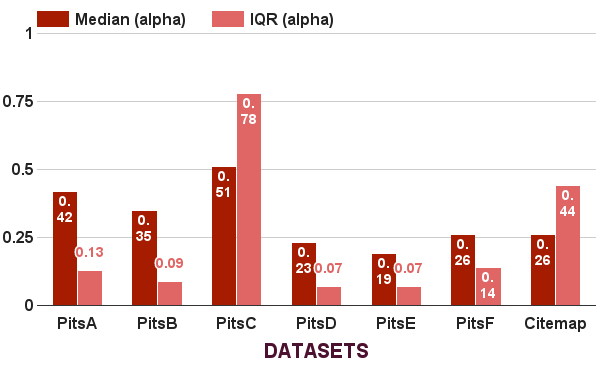
\includegraphics[width=\linewidth]{./fig/Parameters_variation_a.png}
        \caption{Datasets vs Parameter ($\alpha$) variation}
        \label{RQ3:a}
    \end{minipage}
    \begin{minipage}{.33\textwidth}
        \captionsetup{labelsep=space,justification=centering,singlelinecheck=off}
        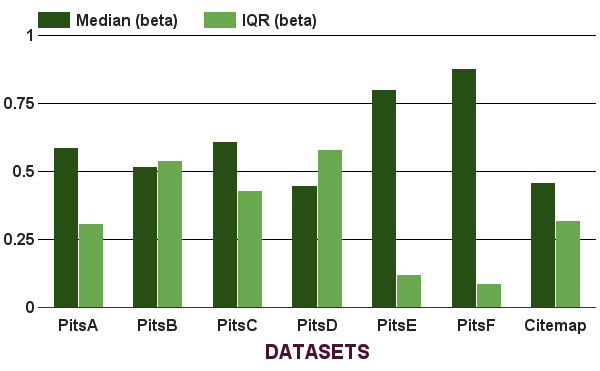
\includegraphics[width=\linewidth]{./fig/Parameters_variation_b.png}
        \caption{Datasets vs Parameter ($\beta$) variation}
        \label{RQ3:b}
    \end{minipage}
\end{figure*}

\begin{figure}[!htbp]
  \begin{center}
    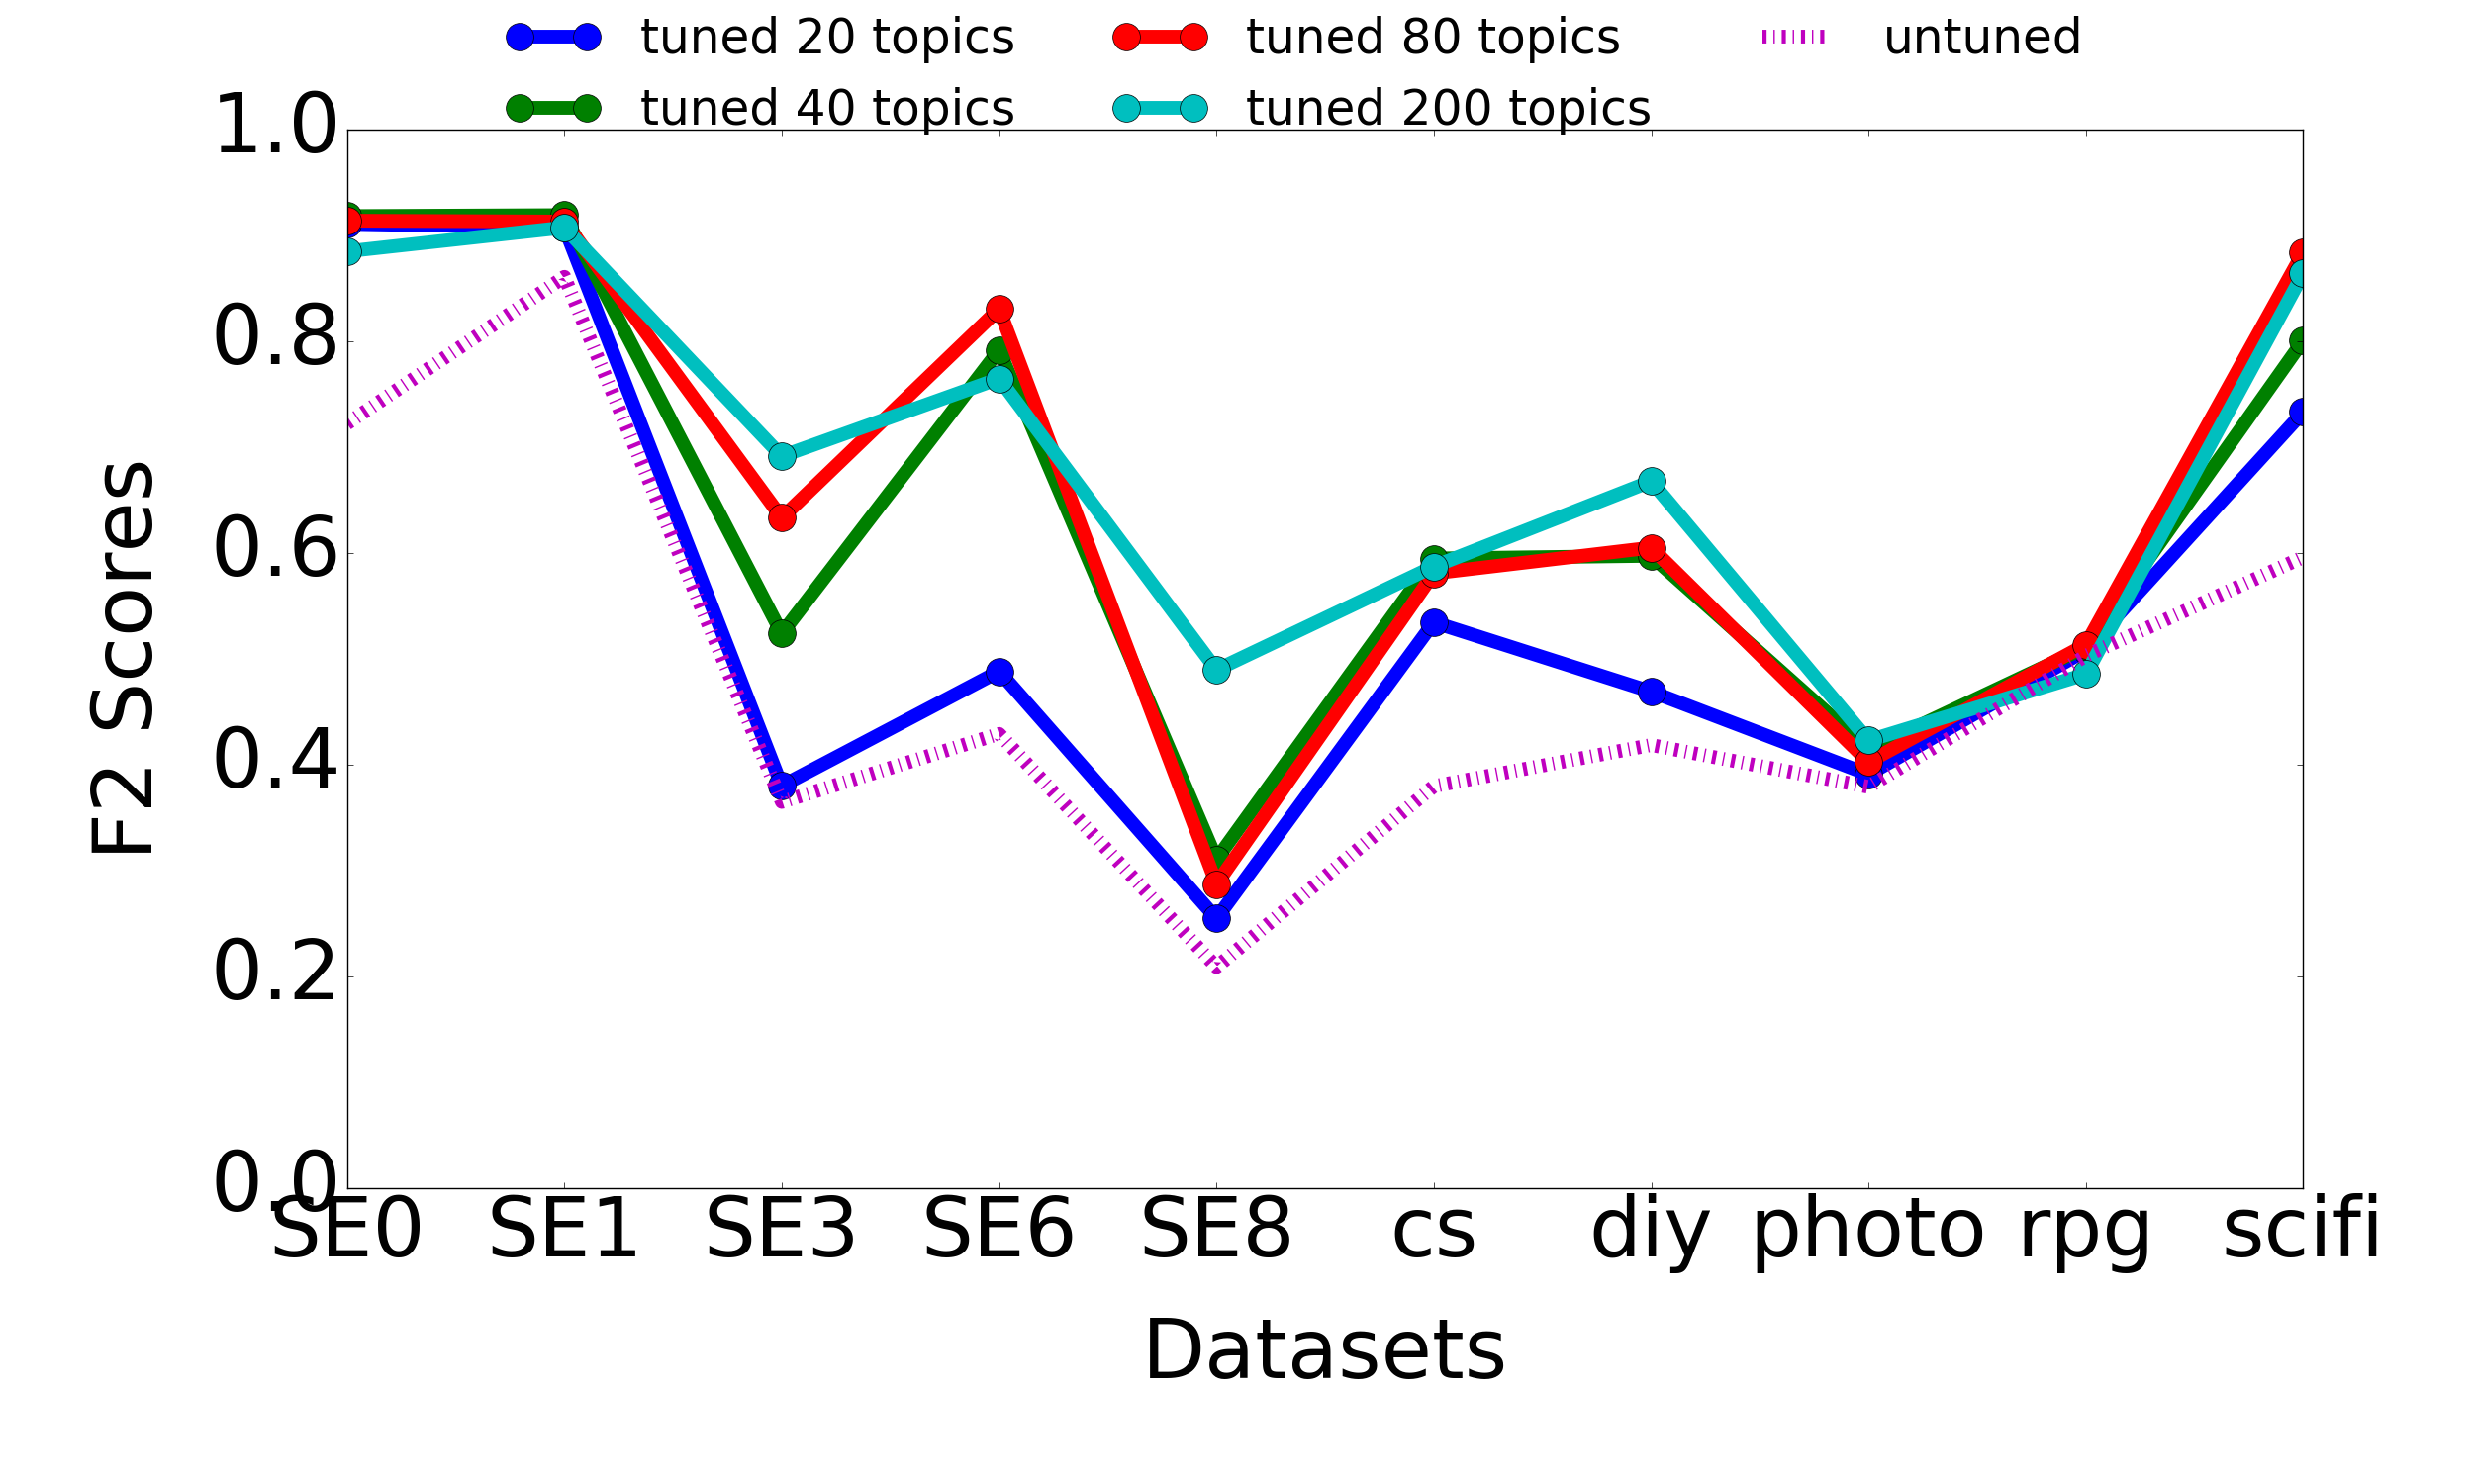
\includegraphics[width=\linewidth]{./fig/classification.png}
    \end{center}
  \caption{Tuning and Untuned results for Classification SE Task}\label{fig:class}  
\end{figure}

\begin{lesson}
For any SE classification task, tuning is again strongly recommended. And $k$ matters the most for a good classification accuracy..
\end{lesson}


\subsection{\textbf{RQ4: Do different data sets
      need different configurations to make LDA stable?}}

Figures \ref{RQ3:k}, \ref{RQ3:a}, and \ref{RQ3:b} show the results of tuning for word overlap of $n=5$.
On display in each set of vertical bars are
the median values generated across 10 tunings.
Also, shown are
the inter-quartile range (IQR) of those tunings (the IQR is the 75th-25th percentile values and is a non-parametric measure of variation
around the median value). Note that in Figure \ref{RQ3:k}, IQR=0 for  PitsB dataset where tuning
          always converged on the same final value.

  These figures
show how tuning selects the different ranges  of
parameters. 
Some of the above numbers are far from the standard values; e.g. Garousi et al~\cite{garousi2016citations} recommend using $k=67$ topics
yet in our data sets, best results were seen using $k \le 24$.
Clearly:

\begin{lesson}
  Do not  reuse tunings suggested by other researchers from other data sets.
  Instead, always retune for all new data.
\end{lesson}
%Our results found out to be quite consistent and all our above research questions results hold valid in these scenarios as well. As to more specific threats to validity, one issue might be that our conclusions on ``LDA'' are really quirks of a specific implementation.

\subsection{\textbf{RQ5}: \textbf{Using different kinds of LDA or with different implementations, are our findings consistent?}}

Results were collected across different implementations of LDA (Python+Scikit-Learn, Scala+Spark); across different platforms (Linux, Macintosh) and for different kinds of LDAs (the traditional VEM method, or using Gibbs sampling). 

To check this, it was insightful to compare our results with:
\bi
\item The Pits and Citemap results, executed in Scikit-Learn and Python running on
  a desktop machine.
\item The StackOverflow data set executed in Scala using Mllib running on a Spark cluster.
  \ei

\begin{figure}[!htbp]
  \captionsetup{justification=centering}
  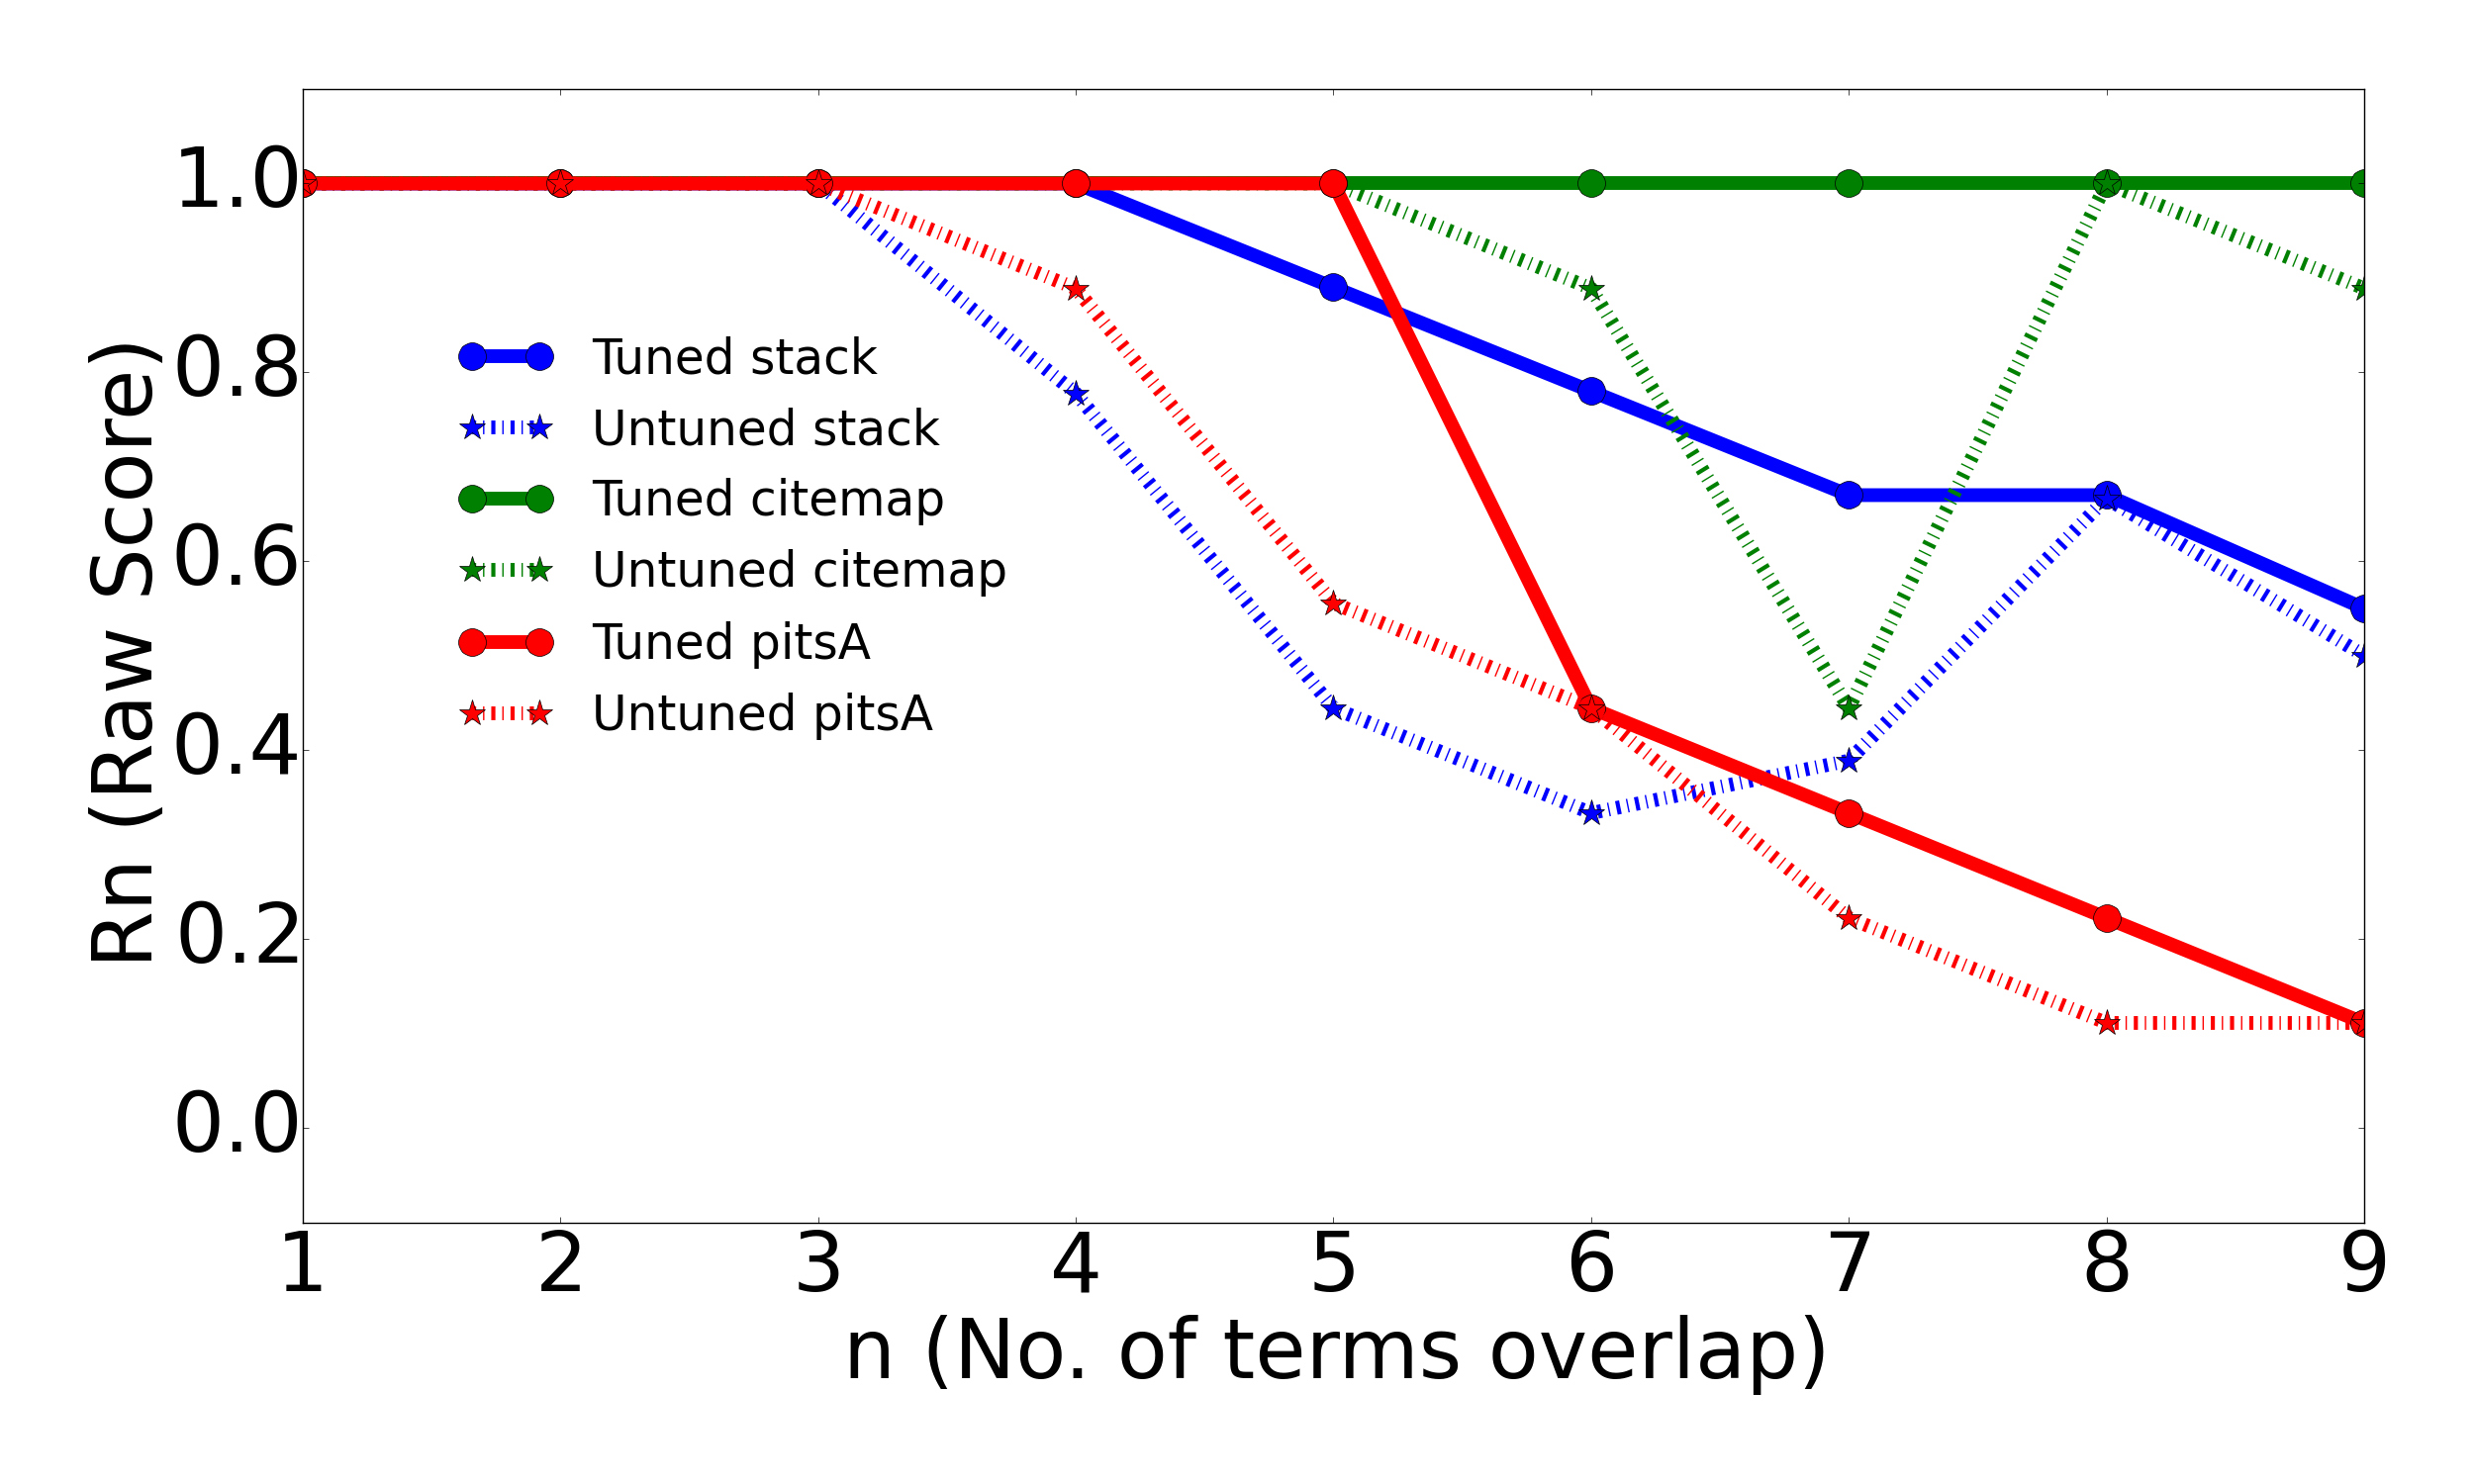
\includegraphics[width=\linewidth]{./fig/spark.png}
  \caption{Spark Results}
  \label{python_spark}
\end{figure}

Figure \ref{python_spark} shows tuning results for StackOverflow, Citemap, and PitsA 
   using Scala/Spark cluster (for results on other data sets, see https://goo.gl/UVaql1).
   
  Another useful comparison is to change the internal of the LDA:
  \bi
\item Sometimes using VEM sampling;
\item Sometimes using Gibbs sampling;
  \ei


\begin{figure}[!htbp]
  \captionsetup{justification=centering}
  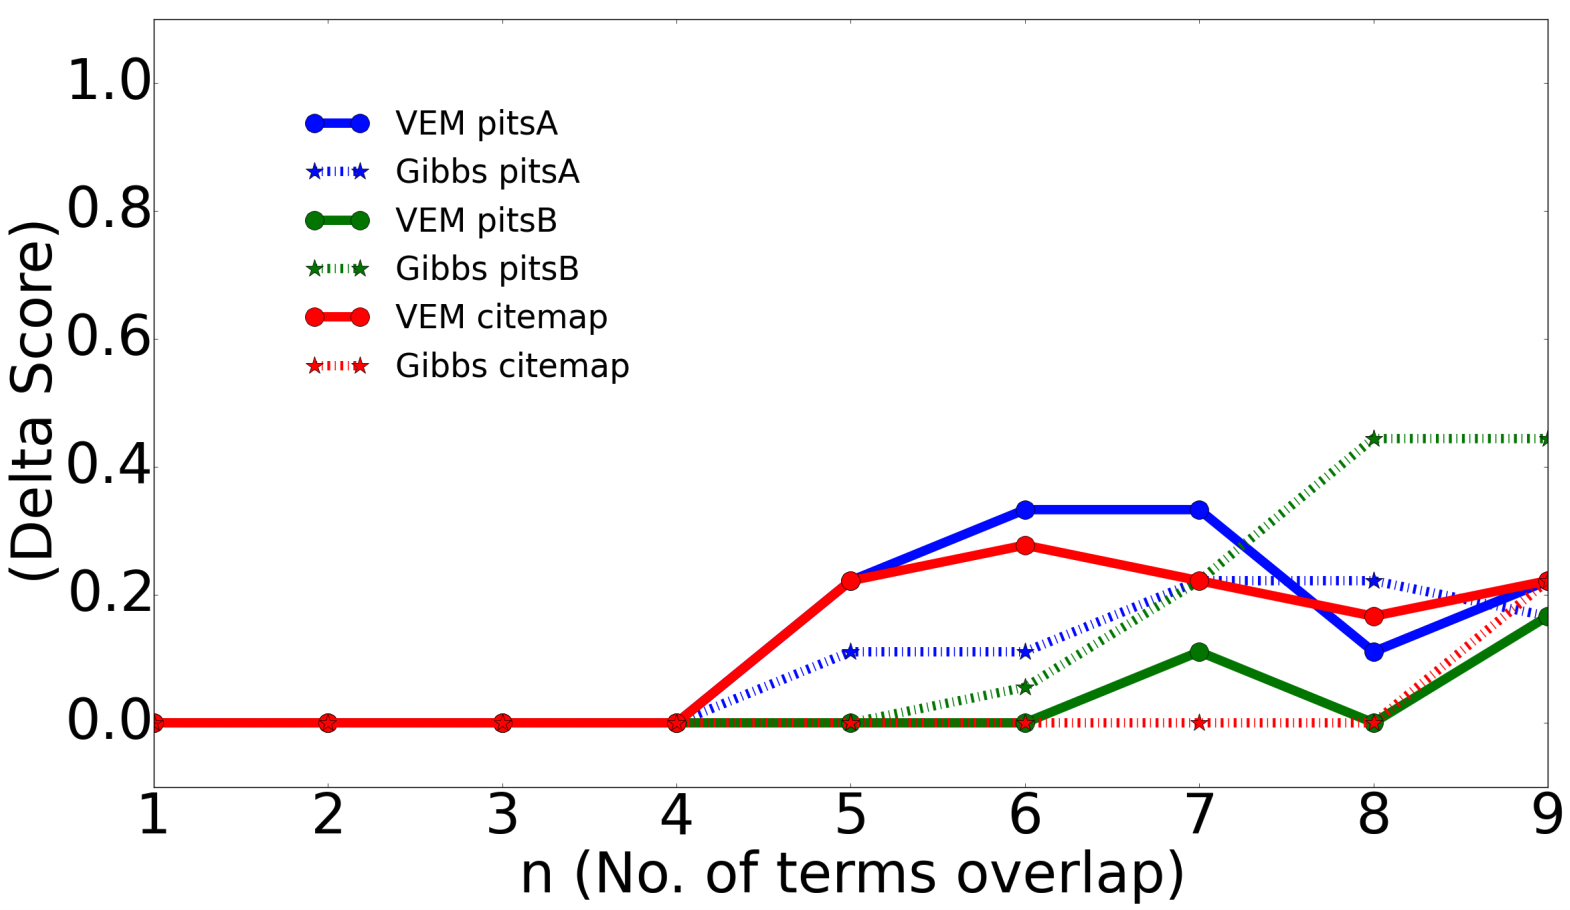
\includegraphics[width=\linewidth]{./fig/gibbs_vem1.png}
  \caption{GIBBS vs VEM}
  \label{gibbs_vem}
\end{figure}


\begin{figure*}[!t]
    \centering
  \begin{minipage}{.49\textwidth}
        \captionsetup{labelsep=space,justification=centering}
        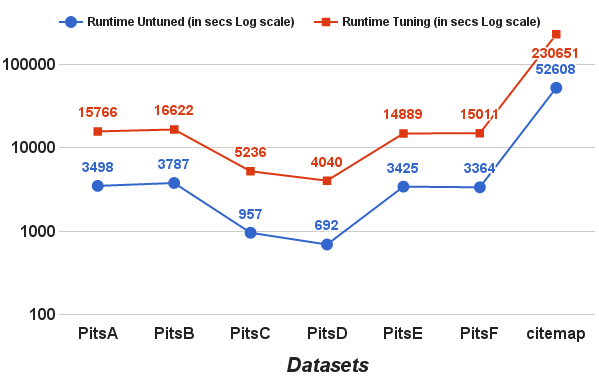
\includegraphics[width=\linewidth]{./fig/Run_VEM_sci.png}
  \caption{VEM: Datasets vs Runtimes}
  \label{RQ5 VEM}
  \end{minipage}
  \begin{minipage}{.49\textwidth}
        \captionsetup{justification=centering}
        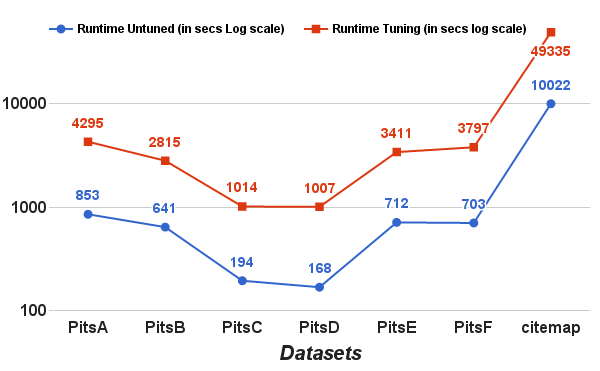
\includegraphics[width=\linewidth]{./fig/Run_gibbs_sci.png}
  \caption{Gibbs: Datasets vs Runtimes}
  \label{RQ5 Gibbs}
    \end{minipage}%
    
\end{figure*}


  Figure~\ref{gibbs_vem} compares the  VEM vs Gibbs sampling (for results on other datasets, see https://goo.gl/faYAcg).
   
   When compared with the Python/desktop results of
   Figure~\ref{fig:delta} we see the same patterns:
   \bi
 \item Tuning never makes stability worse.
 \item Sometimes, it dramatically improves it (in particular, see the Citemap results
   of  Figure~\ref{python_spark}).
   \ei
   That said, there are some deltas between VEM and Gibbs where it seems tuning
   is more important for VEM than Gibbs (evidence: the improvements seen after
   tuning are largest for the  VEM results of  Figure~\ref{gibbs_vem} and at  https://goo.gl/faYAcg).

\begin{lesson}
  Instability is not due to any quirk in the implementation of LDA. Instability is consistent and LDADE can stabilize. 
\end{lesson}

\begin{figure}[!h]
  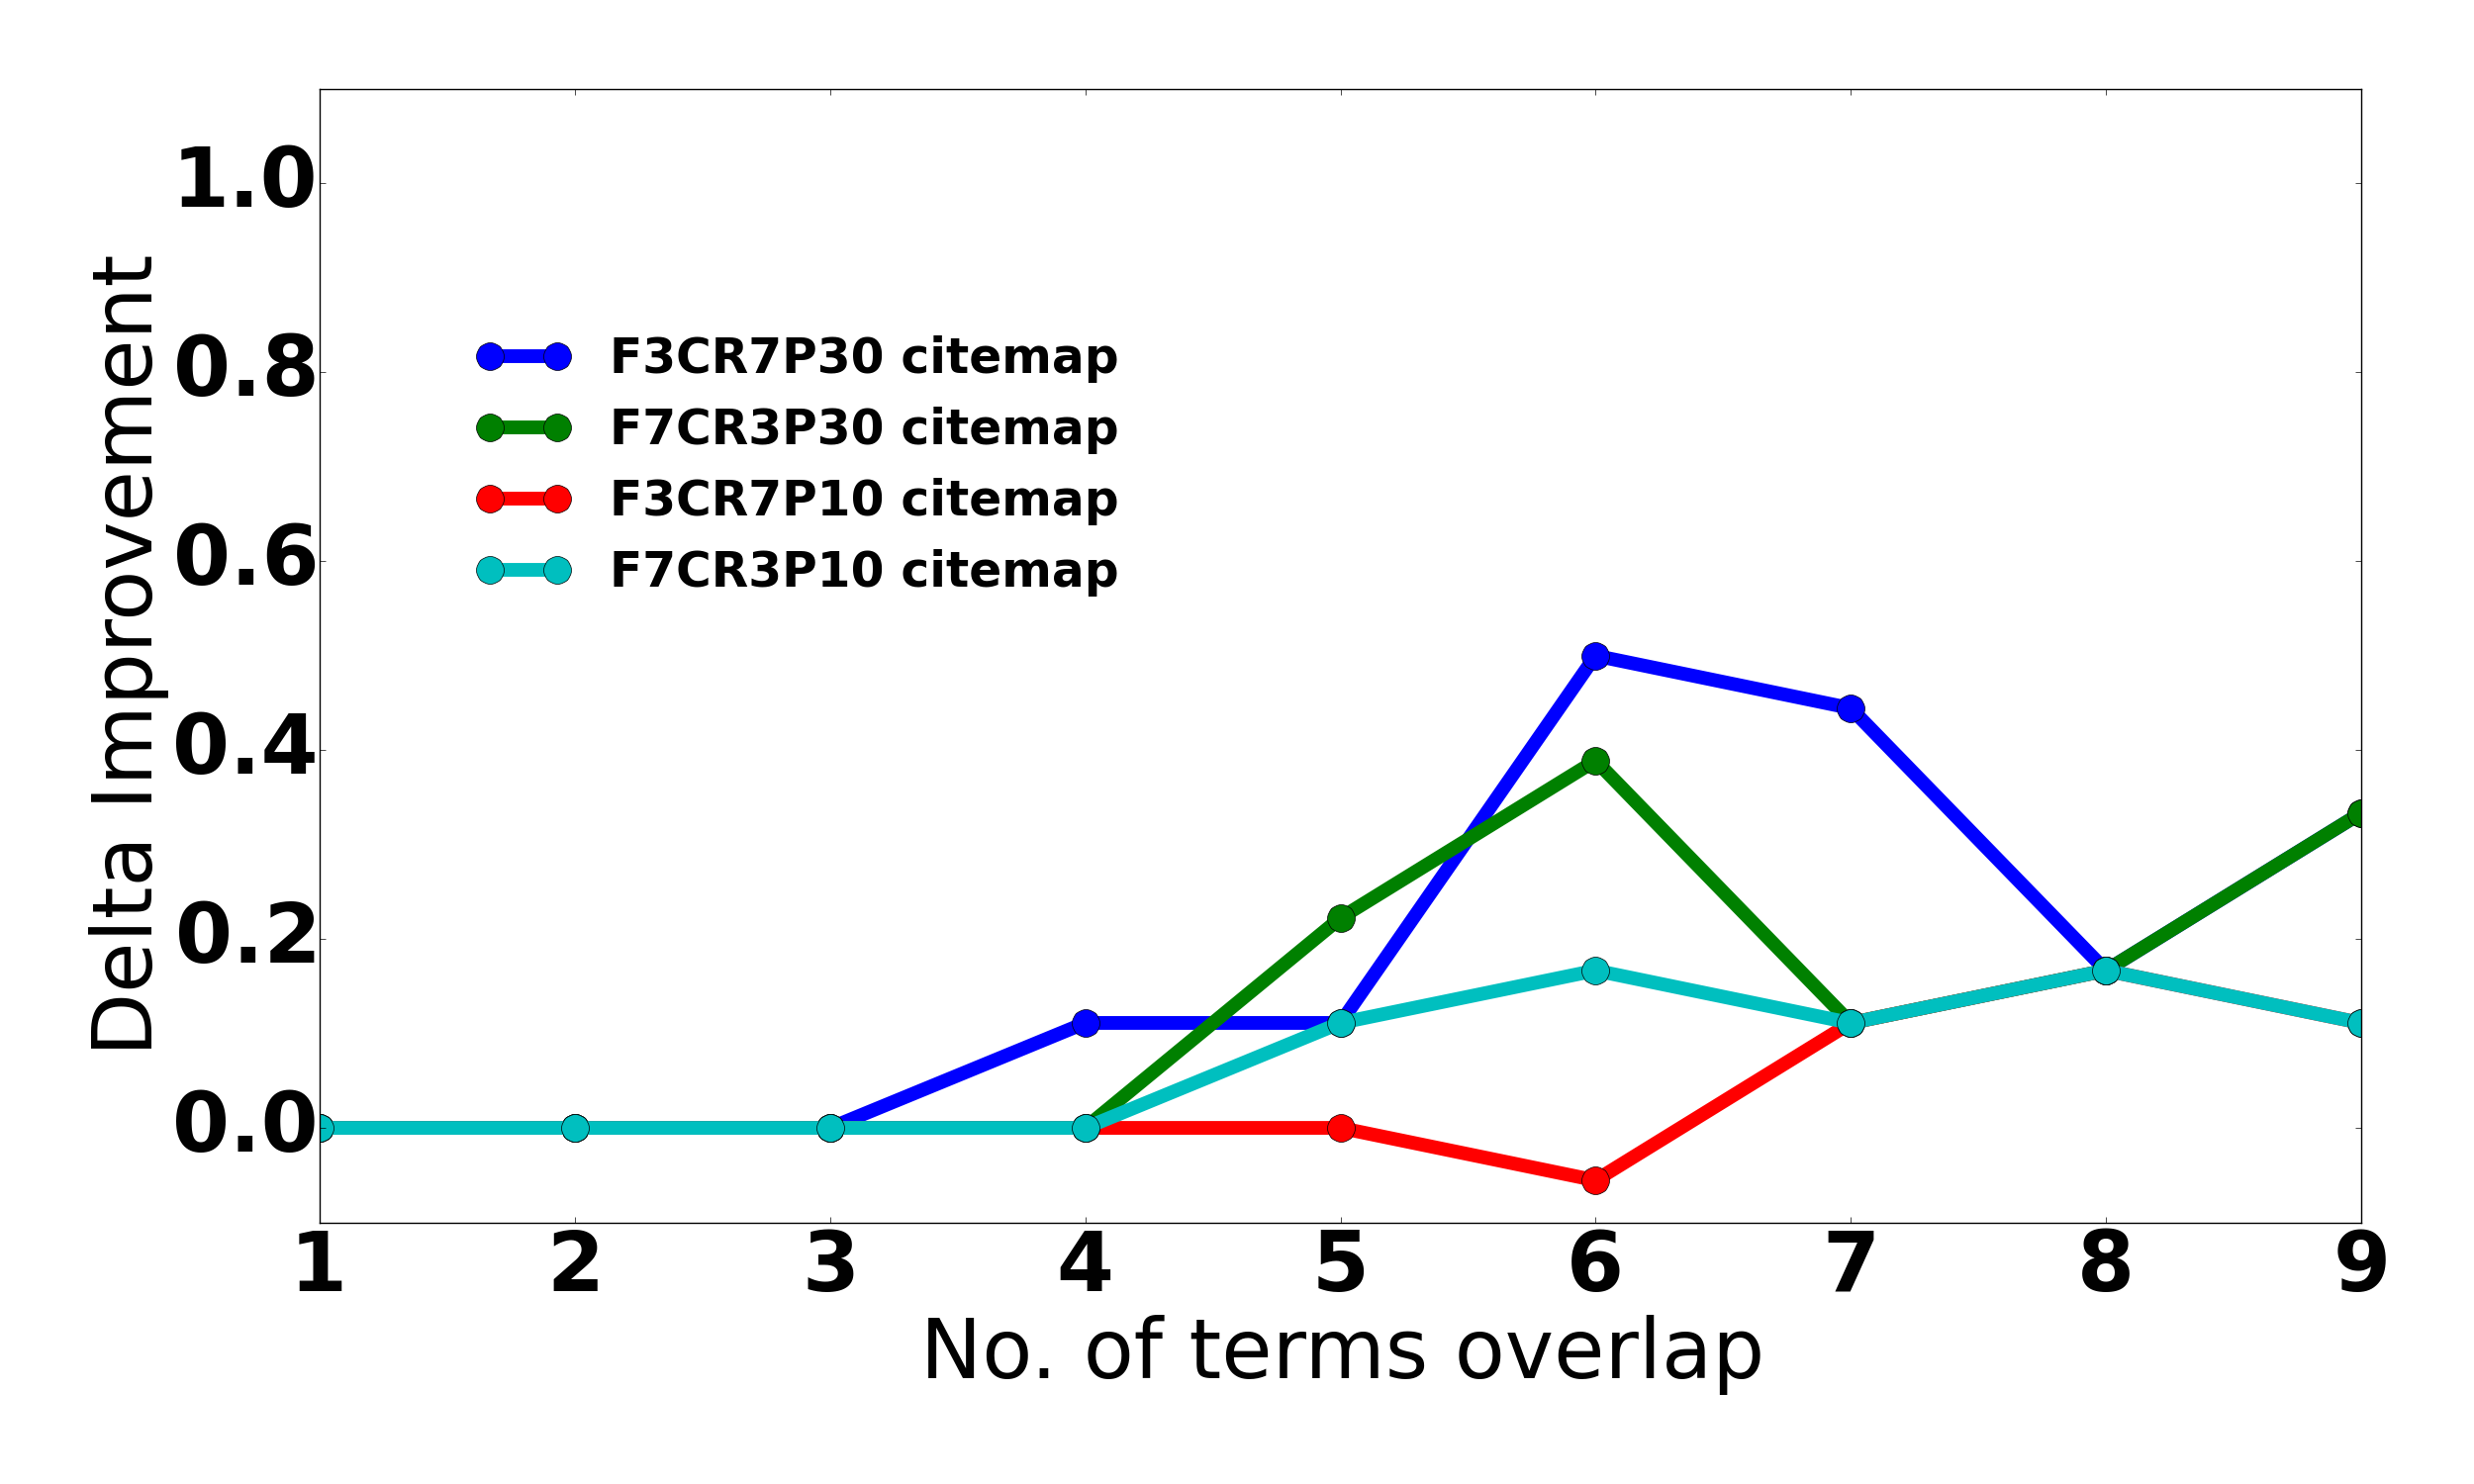
\includegraphics[width=\linewidth]{./fig/citemap.png}
  \caption{Terms vs Delta Improvement using Different settings of DE}
  \label{fig:RQ4}
\end{figure}

\subsection{\textbf{RQ6: Is  tuning  easy?}}


The DE literature
recommends using a population size $np$ that is ten times larger than the number of parameters being
optimized~\cite{storn1997differential}.  For example, when tuning $k,\alpha,\beta$,
the DE literature is recommending $np=30$.
Figure~\ref{fig:RQ4} explores $np=30$ vs the $np=10$ we use in Algorithm 2
(as well as some other variants of DE's F and CR parameters).
The figure shows results just for Citemap and, for space reasons, results
relating to other data sets are shown at https://goo.gl/HQNASF.
After reviewing the results from all the datasets, we can say that there isn't much of an improvement by using different F, CR, and Population size. So our all other experiments used $F=0.7$, $CR=0.3$ and $np = 10$.
Also:

\begin{lesson}
  Finding stable parameters for
  topic models is easier than standard optimization tasks.
\end{lesson}

\subsection{\textbf{RQ7: What is the runtime cost of tuning?}}

Search-based SE methods can be very slow. Wang et al~\cite{wang2013searching} once needed 15
years of CPU time to find and verify the tunings required for software
clone detectors. Sayyad et al~\cite{sayyad2013scalable} routinely used
$10^6$ evaluations (or more) of their models in order to extract
products from highly constrained product
lines. Hence, before recommending any
search-based method, it is wise to consider the runtime cost of that
recommendation.

To understand our timing results, recall that untuned, tuned LDA use
Algorithm~1, Algorithm~2 respectively. Based on the psuedocode
shown above, our pre-experimental expectation is that
tuning will be three times slower than not tuning.
 
Figures \ref{RQ5 VEM} and \ref{RQ5 Gibbs} check if that theoretical
holds true in practice. Shown in blue and red are the
  runtimes required to run LDA untuned, tuned (respectively).  The
  longer runtimes (in red) include the times required for DE to find
  the tunings. Overall, tuning slows down LDA by a factor of up to
  five (which is very close to our theoretical prediction).
  Hence, we say:

  
  \begin{lesson}
    Theoretically and empirically, tuning LDA costs three to five times more runtime
    as much as using untuned LDA.
  \end{lesson}

  While this is definitely more than not using DE, but this may not be an arduous increase
  given modern cloud computing environments.
  

\subsection{\textbf{RQ8: Should data miners be used ``off-the-shelf'' with their default tunings?}}

  Figure~\ref{fig:delta} shows that there is much benefit in tuning.
  Figures \ref{RQ3:k}, \ref{RQ3:a}, and \ref{RQ3:b} show that
  the range of ``best'' tunings is very dataset-specific. Hence, for a new dataset,
  the off-the-shelf tunings
  may often fall far from the useful range.
  Figures \ref{RQ5 VEM} and \ref{RQ5 Gibbs} show that tuning is definitely
  slower than otherwise, but the overall cost is not prohibitive.
  Hence:
  \begin{lesson}
    Whatever the goal is, whether using the learned topics, or cluster distribution for classification
    we cannot recommend using ``off-the-shelf'' LDA.
  \end{lesson}


\section{Threats to Validity}
\label{sect: validity}

As with any empirical study, biases can affect the final
results. Therefore, any conclusions made from this work must be considered with the following issues in mind:

\textbf{\textit{Sampling bias}} threatens any experiment; i.e., what matters there may not be true here. For example,
the data sets used here comes after various pre-processing steps and could change if pre-processed differently. And that is why, the footnotes of this paper contain all the urls where other researchers can download
our datasets and explore the conclusions of this paper. Even though we used so many data sets, there could be other datasets for which our results could be wrong or have lesser improvement.

\textbf{\textit{Learner bias}}: For running LDA, we selected other parameters as default which are of not much importance. But there could be some datasets where by tuning them there could be much larger improvement. And for RQ2, we only experimented with linear kernel SVM. There could be other classifiers which can change our conclusions. Data Mining is a large and active field and any single study can only use a small subset of the known data miners.

\textbf{\textit{Evaluation bias}}: This paper uses Jaccard similarity ($\Re_n$) and F2 measures of evaluation but there are other measures which are used in software engineering which
includes perplexity, fscore, recall, performance. Measuring performance with more measures is left for future work.

\textbf{\textit{Order bias}}: With each dataset, how data samples are picked and put into LDA is completely random. Since this paper also consider input order effects, though there could be times when the input order could be with lesser variance. To mitigate this order bias, we ran the experiment 10 times by randomly changing the order of the data samples each time.


Another threat to validity of this work is that it is a quirk of the control
parameters used within our DE optimizer.
We have some evidence that this is not the case.
Figure~\ref{fig:RQ4} and https://goo.gl/HQNASF explored a range of DE tunings and found
little difference across that range. Also, Table~V explores another choice within DE -- how
many evaluations to execute before terminating DEs. All the results in this paper use an
evaluation budget of 30 evaluations. Table~V
compares results across different numbers of evaluations. While clearly,
the more evaluations the better, there is little improvement after the
30 evaluations used in this paper.

\begin{table}[!htbp]
\begin{center}
\begin{tabular}{|c|c|c|c|c|}
\hline 
\textbf{Datasets\textbackslash Evaluations} & \textbf{10} & \textbf{20} & \textbf{30} &
\textbf{50} \\[0.5ex]
\hline
PitsA & 0.9 & 0.9 & 1.0 & 1.0\\ 
\hline
PitsB & 0.9 & 0.9 & 0.9 & 1.0 \\
\hline
PitsC & 0.9 & 1.0 & 1.0 & 1.0\\ 
\hline
PitsD & 0.9 & 1.0 & 1.0 & 1.0\\ 
\hline
PitsE & 0.9 & 0.9 & 1.0 & 1.0\\
\hline
PitsF & 0.9 & 0.9 & 0.9 & 0.9\\
\hline
Citemap & 0.67 & 0.67 & 0.77 & 0.77\\
\hline
StackOverflow & 0.6 & 0.7 & 0.8 & 0.8\\
\hline
\end{tabular}
\end{center}
\caption{Evaluations vs Stability Scores}
\label{tb:tablename1}
\end{table}

The conclusions of this paper are based on a finite number of data sets and it is possible
that other data might invalidate our conclusions. As with all analytics papers, any researcher can do is to make their conclusions and materials public, then encourage
other researchers to repeat/ refute/ improve their conclusions. For example, the footnotes of this paper contain all the urls where other researchers can download
our materials and explore the conclusions of this paper.

\section{Conclusion and Future Work}

Based on the above, we offer a specific and general conclusion. Most specifically, we recommend 
\begin{itemize}

\item  
Any study that shows the topics learned from LDA, and uses them to make a particular
conclusion, needs to first tune LDA. We say this since the topics learned from untuned LDA are unstable, i.e. different input orderings will lead to different conclusions. However, after tuning, stability can be greatly increased.
\item Unlike the advise of Lukins et al~\cite{lukins2010bug}, LDA topics should not be reported as the top ten words.
  Due to order effects, such a report can be highly incorrect.
  Our results show that up to eight words can be reliably reported, but only
  after tuning for stability using tools like LDADE.
 \item Any other studies which are making use of these topic distribution for classification results need to be tuned first before using them in their further tasks.
\item Do not download someone else's pre-tuned LDA since, as shown here,  the best LDA tunings vary from data set to data set.
\item These results demand us to visit the previous case studies which have used LDA using ``off-the-shelf parameters to rerun by tuning these parameters using automated tools like LDADE.
    
\end{itemize}
Our experience is that this recommendation is not an arduous demand since tuning adds less than a factor of five to the total run times of an LDA study.

More generally, we comment that the field of software analytics needs to make far more use of search-based software engineering in order
to tune their learners. In other work, Fu et al have shown that tuning significantly helps defect prediction~\cite{fu2016tuning} (a result that has also been reported by
other researchers~\cite{panichella2013effectively}). In this work, we have shown that tuning significantly helps topic modeling by mitigating a systematic error in LDA  (order effects that lead to unstable topics). The implications of this study for other software analytics tasks is now an open
and pressing issue. 
In how many domains can search-based SE dramatically improve software analytics?


\section*{Acknowledgements}
		The work is partially funded by NSF award \#1506586.
	
\balance


\bibliographystyle{elsarticle-num}
\medskip
\bibliography{main}

\end{document}
